\includeonly{settings,HandbuchInc,titel,Kapitel1,Kapitel2,Kapitel3,Kapitel4,Kapitel5,Kapitel6,Quelltexte,ErstellungEigenerMatches,Erklaerung}
\documentclass[a4paper,12pt,twoside,halfparskip,bibtotocnumbered,liststotocnumbered]{scrreprt}

\usepackage{ngerman}	%Deutsch
\usepackage[T1]{fontenc}
\usepackage[utf8]{inputenc}
\usepackage[german]{varioref}
\usepackage{gensymb}	%Sonderzeichen
\renewcommand{\baselinestretch}{1.05}
\usepackage{index}

\usepackage{subfigure}

\newindex{default}{idx}{ind}{E Stichwortverzeichnis}

  
\usepackage{amsmath}	%MAthe
\usepackage{amsfonts}
\usepackage{amssymb}

\usepackage{listings}	%für Quellcode
\usepackage{xcolor}	%für Farben im Quellcode
\lstset{language=[gnu]c++}%language=java}
\lstset{alsolanguage=Java}
\lstset{inputencoding=utf8,
        extendedchars=\true }
\lstset{emph={HashSet,RegionForInterpolation,Face, ConvexHullTreeNode,RegionTreeNode, CHLine, LineDist,LineWA}}
\lstset{morekeywords={NULL}}
\lstset{stringstyle=\color{blue}}
\lstset{keywordstyle=\color{magenta}\textbf}
\lstset{commentstyle=\color{green}\itshape}
\lstset{breaklines=true,frame=tlrb,frameround=tttt,rulecolor=\color{black},numbers=left,emphstyle=\color{red}\textbf,tabsize=3}

\usepackage{bibgerm}
\usepackage{graphicx}
\usepackage{picins}
\usepackage{ifpdf}
\ifpdf
\DeclareGraphicsRule{*}{mps}{*}{}
\fi

\usepackage{multicol}
\usepackage[german,vlined,boxruled,algochapter]{/usr/local/teTeX/share/texmf-dist/tex/latex/algorithms/algorithm2e}
\setlength{\algomargin}{1em}
%&\SetInd{1em}{1em}
\Setvlineskip{1em}
\usepackage{framed}
\usepackage{lscape}

\usepackage{units}	%\usepackage{units} 	  	units → Paket für Einheiten: mit \unit[wert]{einheit}, Bsp.: 5 mm \unitfrac[wert]{zähler}{nenner}, Bsp.: 5 g/m \nicefrac[schrift]{zähler}{nenner}

\usepackage[germanb]{minitoc}
\mtcsettitle{parttoc}{Anhangsverzeichnis}
\mtcsetdepth{parttoc}{0}
\mtcsetrules{*}{off} 
\setcounter{tocdepth}{1} %% <- Tiefe bei (Haupt-)Inhaltsverzeichnis

\usepackage{fancyhdr} % für spezielle Kopfzeilen
\usepackage{floatflt}
\pagestyle{fancy}
\setlength{\headheight}{12mm}
\addtolength{\headwidth}{\oddsidemargin}
\addtolength{\headwidth}{\evensidemargin}
\fancyhead[ER,OL]{
\includegraphics[height=1cm]{/home/java/Documents/Tex/Tex/feu_logo2.eps}}
\renewcommand{\chaptermark} [1]{\markboth{ \thechapter.  #1}{ \thesection   #1}}
\fancyhead[EL]{\sc\leftmark }
\fancyhead[OR]{\sc\rightmark}
\lfoot[\thepage]{}
\rfoot[]{\thepage}
\cfoot{}
\renewcommand{\labelenumi}{\theenumi)}
\renewcommand{\labelenumii}{(\alph{enumii})}
\definecolor{red}{rgb}{1,0,0}
\definecolor{RED}{rgb}{1,0,0}
\newcommand{\anmerkung}[1]{{\textit{#1}}}


\usepackage[
dvipdfm,
raiselinks=false,
pdfdisplaydoctitle=true,
breaklinks=true,
 pdfpagelabels=true,
 bookmarks=true,
colorlinks=true,
linkcolor=black,
anchorcolor=black,
citecolor=black,
filecolor=black,
menucolor=black,
urlcolor=black]{hyperref}

\hypersetup{% ä=\344, ö=\366, ü=\374, Ä=\304, Ö=\326, Ü=\334, ß=\377
 pdftitle={Berechnung beweglicher Objekte aus Beobachtungen},
 pdfauthor={Andreas Ruloffs},
 pdfsubject={},
 pdfkeywords={},
 pdfcreator={LaTeX},
 pdfproducer={LaTeX mit hyperref}
}

\begin{document}
%
%       titel.tex - Titelblatt
%
% --- ! Anpassungen sind nur GANZ UNTEN erforderlich !  ---
%
% ---------------------------------------------------------
%       Diese Datei ist Teil der LaTeX-Vorlage fr
%             Studien-und Diplomarbeiten am
%    Institut fr Mechanik und Meerestechnik, TUHH
%
% (c) Institut fr Mechanik und Meerestechnik
%     Technische Universit� Hamburg-Harburg
%     2006
%
% Weitere Informationen finden Sie in  diplomarbeit.tex .
% ---------------------------------------------------------
%
%

% ------------ Definition der Befehle ---------------
%       (hier sind keine Aenderungen noetig !)

% \deckblatt{Rand}{Seitenbreite}{Kopftext}{Fensterbreite}{Fensterhoehe}{Fenstertext}{Untertext}{Fusstext}
%
% Rand:          zusaetzlicher rechter Rand zur Ausrichtung der Seite auf das Sichtfenster
% Seitenbreite:  Seitenbreite
% Kopftext:      Text ueber dem Sichtfenster
% Fensterbreite: Breite des Sichtfensters
% Fensterhoehe:  Hoehe des Sichfensters
% Fenstertext:   Text im Sichtfenster
% Untertext:     Text unter dem Sichtfenster
% Fusstext:      Text nach \vfill

\newcommand{\deckblatt}[8]{
  \begin{titlepage}
  \vspace*{-20mm}
  \hspace{#1}               % Ausrichtung zum Sichtfenster, auch unten
  \begin{minipage}[t]{#2}       % Minipage Titelseite
    \begin{center}
    \begin{minipage}[t][64mm][t]{#2}    % Minipage Kopf
      \begin{center}
      #3
      \end{center}
    \end{minipage} \\           % Minipage Kopf
    \vspace{10mm}
    \begin{minipage}[t][#5][c]{#4}  % Minipage Sichtfenster
      \begin{center}
      #6
      \end{center}
    \end{minipage} \\           % Minipage Sichtfenster
    \vspace{26mm}
    #7
    \end{center}
  \end{minipage} \\         % Minipage Titelseite
  \vfill
  \hspace{#1}               % Ausrichtung der Titelseite zum Sichtfenster
  \begin{minipage}[t]{#2}      % Minipage Datum
    \begin{flushright}
		#8
	\end{flushright}
  \end{minipage}            % Minipage Datum
  \end{titlepage}
}

% \titelseite{Fenstertext}{Untertext}{Fusstext}

\newcommand{\titelseite}[3]{%
  \deckblatt{1mm}{175mm}{
    \vspace*{15mm}    
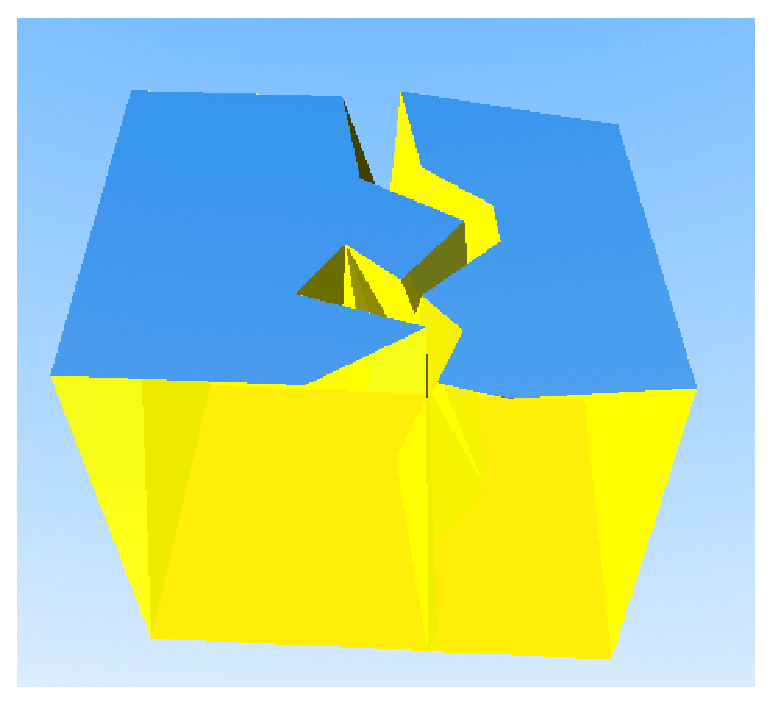
\includegraphics[width=65mm]{/home/java/Documents/Tex/Tex/vrml.eps}
  }{105mm}{65mm}{#1}{#2}{#3}
}

% ------------------ ! Text hier anpassen ! ------------------------

% Schema:  \titelseite{Fenstertext}{Untertext}{Fusstext}
% Fenstertext:   Text im Sichtfenster
% Untertext:     Text unter dem Sichtfenster
% Fusstext:      Text nach \vfill

\titelseite{
  % Fenstertext
  {\large \bf Diplomarbeit} \\  [7mm]
  {\LARGE \bf Berechnung beweglicher Objekte aus Beobachtungen}\\[7mm]
  {vorgelegt von} \\[7mm]
  {\large Andreas Ruloffs}\\
  {\large 6~65~11~19}
}{
  % Untertext
\begin{flushright}
  Betreuer: \\[5mm]
  Prof. Dr.Ralf Hartmut G"uting \\[12mm]
   \begin{floatingfigure}[r]{20mm}
      
\includegraphics[width=20mm]{/home/java/Documents/Tex/Tex/feu_logo2.eps}
   \end{floatingfigure}
\textbf{FernUniversit"at}\\
Gesamthochschule Hagen\\
Fachbereich Informatik\\
Lehrgebiet Praktische Informatik IV
\end{flushright}
}{
  % Fusstext
 Gelsenkirchen, Mai 2008}

%\begin{abstract}
%Diplomarbeit halt
%\end{abstract}
\dominitoc[e]
\doparttoc

\tableofcontents 
%\vfill
%\begin{verse}
%Oftmals wollt ich schon verzagen,\\
%und ich dacht ich trüg es nie,\\
%und ich hab es doch getragen,\\
%aber fragt mich nur nicht wie!\\
%\end{verse} 
%\textbf{Heinrich Heine}
%


\chapter[Einleitung \anmerkung{ca. 5 Seiten}]{Einleitung\\
\normalsize{(kuze Einleitung, was ist Secondo, warum MovinRegions, warum Interpolation) \anmerkung{ca. 5 Seiten}}} \label{Kapitel1}
\anmerkung{Beschreibung der allgemeinen Problemstellung, man m"ochte Moving-Regions darstellen k"onnen z. B. f"ur die Deter Daten, Kurzbeschreibung dieser Daten, das f"uhr zu Secondo, und den Moving-Regions in Secondo. Die Schwierigkeiten bie der Erstellung von diesen, und die Struktur der Deter-Daten f"uhren zu dem Interpolations-Problem, dass im folgenden gel"oste dwerden soll.}


%\minitoc
%\newpage
%\section{Secondo \anmerkung{2 Seiten}}
%\subsection{Was ist Secondo}
%\anmerkung{Eine kuze Beschreibung, was Secondo ist, Die Entstehungsgeschichte und was Secondo so alles kann.}
%\section{Moving Regions \anmerkung{2 Seiten}}
%\anmerkung{Eine kurze Beschreibung, was Moving-Regions sind, und eine Beschreibung wozu diese gut sind. Eventuell k"onnte ich %hier das Flugzeugbeispiel benutzen}
%\subsection{Was sind Moving Regions?}

%\subsection{Wof"ur sind Moving Regions gut?}

%\section{Interpolation \anmerkung{1 Seite}}
%\anmerkung{Warum die Erzeugung von Moving-Regions kompliziert ist, und inwiefern diese Problemetik sich duch meine Arbeit verbesesrn wird.}
%\subsection{Was sind die Probleme bei der Erstellung von Moving Regions?}
%\subsection{Wie sieht die L"osung aus?}

\chapter[Darstellung der Grundlagen \anmerkung{30-40 Seiten}]{Darstellung der Grundlagen\\
\normalsize{(nicht selbstgemachtes
Secondo,
MovingRegion,
T\o{}ssebro)}\anmerkung{30-40 Seiten}} \label{Kapitel2}
\minitoc
\newpage
\section{Secondo \anmerkung{10 Seiten}}\label{SecondoEinfuehrung}
\anmerkung{Eine ausf"uhlichere Beschreibung von Secono, speziell des Konzeptes der Algebren, und eine Beschreibung der Algebren ,,Spatial-Algebra'' und ,Moving-Region-Algebra''.}
\subsection{Das Konzept der Secondo-Algebren}
\subsection{Spatial-Algebra}
\subsection{Moving-Region-Algebra}

\section{Das Paper von Erlend T\o{}ssebro \anmerkung{10 Seiten}}\label{Tossebro}

Eine der wichtigsten Grundlagen der vorliegenden Arbeit ist das Paper: ,,Creating Repesentations for Continuously Moving Regions from Observations'' \cite{TG} von Erlend T\o{}ssebro und Ralf Hartmund G"uting \cite{TG}, in dem die Autoren sich mit den theoretischen Grundlagen des Problems besch"aftigt, und L"osungsvorschl"age zu vielen der vorkommenden Teilprobleme gemacht haben.

Im Rahmen dieses Projektes ist auch eine Java-Applikation entstanden, welche im Rahmen meiner Arbeit erweitert wurde.

\subsection{Die zugrundeligenden Datentypen}
Nach der allgemeinen Einleitung skizzierten die Autoren kurz die Datentypen, wie diese in \cite{FGNS} beschrieben sind.

Zuerst die nicht beweglichen Daten:
$$Seg=\{(u,v)|u,v\in Point, u<v\}$$

Ein Segment ist also ein Liniensegment zwischen zwei Punkten. 

$$Cycle=\{S\subset S\}$$

Ein Cycle ist eine Menge von Liniensegmenten, die zusammen ein einfaches Polygon bilden müssen.

$$Face=\{(c,H)|c\in Cycle, H \subset Cycle\}$$

Ein Face setzt sich aus einem Cycle, der äußeren Begrenzungslinie, und einer Menge von anderen Cycles, den Löchern oder Holes zusammen. Jedes Hole muss komplett innerhalb des äußeren Cycles liegen, und zwei Holes dürfen sich nicht überschneiden. 

$$Region=\{F\subset Face|f_1,f_2\in F \wedge (f_1\neq f_2) \Rightarrow \text{Kanten von }f_1\text{ und } f_2 \text{ sind disjunkt. } \}$$

Eine Region schließlich setzt sich aus mehreren Faces zusammen, wobei sich diese nicht überschneiden dürfen. 

Nun skizzieren die Autoren die beweglichen Datentypen:

$$MPoint=\{(x_0,x_1,y_0,y_1)|x_0,x_1,y_0,y_1\in \mathbb{R}\}$$

Ein MovingPoint setzt sich aus zwei Punkten, dem Start- und dem Endpunkt zusammen.

$$MSeg=\{(s,e)|s,e\in MPoint\}$$

Ein MovingSegment setzt sich aus zwei MovingPoints zusammen, wobei aber alle vier beteiligten Start- und Endpunkte auf einer Ebene liegen müssen. Ein wichtiger Sonderfall des MovingSegemnts ist der, wenn beide Start- oder beide End-punkte zusammenfallen. In diesem Fall repräsentiert ein MovingSegment ein Dreick in drei Dimensionen.

$$MCycle=\{(s_0,s_1,\hdots ,s_{n-1})|n\geq3, s_i\in MSeg\}$$

Ein MovingCycle ist die bewegliche Version eines Cycles. Die beteiligten MovingSegemnts müssen zusammen eine geschlossene, dreidimmensionale Struktur bilden.

$$MFace=\{(c,H)|c\in MCycle, H\subset MCycle\}$$

Ein MovingFace ist die dreidimensionale Version eines Faces, und setzt sich analog zu diesem zusammen.

$$URegion=\{(i,F)|i\in Intervall, F\subset MFace\}$$

Eine RegionUnit schließlich besteht aus einer Menge von MovingFaces und einem Zeitintervall. 

Eine MovingRegion schließlich besteht aus mehreren RegionUnits, bei denen die Zeitintervalle paarweise disjunkt sind.

\subsection{Der Rotating-Pane-Algorithmus}

Die Autoren entwickeln einen Algorithmus, mit dessen Hilfe sich MovingCycles aus zwei konvexen Polygonen berechnen lassen. Anschaulich funktioniert dieser Algorithmus wie folgt:

Wähle eine Kante $s$ des einen Polygons, und lasse die Grundebene des Polygons entlang dieser Achse rotieren. Die Ebene wird dann auf das andere Polygon treffen. Trifft die Ebene zuerst auf einen einzigen Punkt $T$, so gehört das Dreick aus den beiden Punkten von $s$ und $T$ zu dem MovingCycle.

Trifft die Ebene aber auf eine Kante $t$, so gehört das MovingSegment von $s$ zu $t$ zu dem MovingCycle.

Dieses Verfahren wende auf alle Kanten aus beiden Polygonen an.

Die Autoren geben auch noch einen Algorithmus an, der diese Idee weiterverfolgt, der aber technisch einfacher zu implementieren ist. Eine leicht veränderte Version dieses Algorithmuses beschreibe ich unter \ref{rotPane} genauer.

Die Autoren geben noch die Laufzeit des Verfahrens an und sagen, dass der Algorithmus zu zwei Polygonen, welche zusammen $n$ Ecken haben, ein MovingCycle berechnet und hierfür $O(n*\log{n})$ Zeit benötigt. Liegen die Punkte der Polygone bereits sortiert vor, so sinkt die Laufzeit auf $O(n)$.

Die Autoren räumen ein, dass dieses Verfahren nicht gut mit Rotationen umgehen kann. Lassen wir etwa zwei dünne Rechteck durch diesen Algorithmus laufen, die um 90\degree gedreht sind, so wird die Interpolation nach der Hälfe der Zeit ungefähr quadratisch  sein und einen zu großen Flächeninhalt aufweisen. Abbildung~\ref{fig:BeispielschlechteRot} zeigt dieses Beispiel. Eine Lösung dieses Problems können die Autoren nicht angeben, bei Rotationen sollten also die Unterschiede zwischen den Schnappschüssen nicht zu groß sein.

\begin{figure}
	\centering
	
\includegraphics{feu_logo2.eps}
	\caption{Ein Beispiel in dem man die Schwäche des Verfahrens bei großen Rotationen zeigt.}
	\label{fig:BeispielschlechteRot}
\end{figure}

\subsection{Der Konvexe Hüllenbaum}

Das obige Verfahren kann nur mit konvexen Polygonen umgehen. Um im Allgemeinen einfache Polygone bearbeiten zu können führen die Autoren den ConvexHullTree ein. Die Idee hinter diesen ist es, einfache Polygone als konvexe Polygone mit konvexen Löchern aufzufassen. 

Ein ConvexHullTreeNode ist ein konvexes Polygon, bei dem jeder Kante wiederum ein ConvexHullTreeNode zugeordnet werden kann. Diese Kinderelemente werden von dem Vaterelement abgezogen. Abbildung~\ref{fig:ConHullTree} zeigt einen solches Konstrukt.

\begin{figure}
	\centering
	
\includegraphics{feu_logo2.eps}
	\caption{Ein Beispiel für einen ConvexHullTree.}
	\label{fig:ConHullTree}
\end{figure}

Die Autoren beschreiben, wie man einen solchen Baum aufbaut. Dieses Verfahren ist näher unter \ref{constCHTN} beschrieben.

Die Komplexität der Konstuktion eines Hüllenbaumes wird mit $O(dn*\log(n))$ angegeben, wobei $d$ die Tiefe des resultierenden Baumes ist.

Der umgekehrte Weg, also aus einem ConvexHullTee wieder ein Polygon zu erzeugen funktioniert so:

\begin{itemize}
\item Gebe jedes Segment zurück, für das es kein Kindelement gibt.
\item Für jedes Segment, welches ein Kindelement hat benutze diese Funktion rekursiv.
\end{itemize}

\subsection{Matching zweier Regionen}

Im Weiteren beschäftigen sich die Autoren mit der Frage, wie man zu gegebenen Polygonen, welche die beiden Schnappschüsse einer MovingRegion darstellen sollen, ein Match bestimmen kann. Ein Match ist eine Menge von Paaren von Cyclen, die zusammengehören.

Die Autoren unterscheiden drei unterschiedliche Arten von Matches:

\begin{itemize}
\item Wenn beide Regionen aus mehreren Faces zusammengesetzt sind, welche Faces auf der einen Seite passen dann zu welchen Faces auf der anderen Seite?
\item Falls ein Face mehrere Holes hat, welches Hole auf der einen Seite passt dann zu welchem Hole auf der anderen Seite?
\item Hat ein Cycle mehrere Konkativitäten, welche Konkativitäten auf der einen Seite passen dann zu welchen Konkavitäten auf der anseren Seite?
\end{itemize}

In all diesen Fällen ist auch noch zu beachten, dass einzelne Objekte verschwienden können, oder das mehrere auf der einen Seite zu einem Objekt auf der anderen Seite verschmelzen können.

Um die Qualität eines Matches bestimmen zu können, geben die Autoren einige Kriterien an:

\begin{enumerate}
\item Ein matching-Verfahren sollte das korrekte Ergebnis liefern, falls beide Schnappschüsse übereinstimmen.
\item Komponenten, die sich relativ zu ihrer Größe wenig bewegt haben, sollten korrekt gematcht werden können.
\item Komponenten die nur kleine Änderungen an Größe und Form erfahren haben sollten korrekt gematcht werden.
\item Ein Matching-Verfahren sollte Komponenten erkennen, die sich in mehrere neue aufgesplittet haben, oder solche die sich vereinigen.
\item Ein Matching-Verfahren sollte Kriterien anbieten um zu entscheiden, ob zwei Momentaufnahmen gut zueinander passen, oder ob der zeitliche Abstand zwischen diesen zu groß gewählt ist.
\end{enumerate}

Die Autoren führen den Begriff des ,,sicheren'' Matches an:

Sei $mr$ eine MovingRegion und seien $S_1$ und $S_2$ zwei Schnappschüsse dieser MRegion zu den Zeitpunkten $t$ und $t+\Delta t$. Ein Matching-Verfahren ist sicher zu nennen, falls es ein $\epsilon >0$ gibt, so dass das Match korrekte Ergebnisse liefert, für alle $\Delta t < \epsilon$.

Die Autoren finden drei verschiedene Matching-Strategien, die im folgenden kurz aufgef"uhrt werden:
\begin{enumerate}
\item Position of centroid \label{MatchSchwer}

Bestimme den Schwerpunkt jedes Cycles,  bilde aus diesem einen gewichteten Graphen, mit den Entfernungen als Kantengewichte und suche in diesem "`N"achste Nachbarn"'.
\item Fixed threshold (set of cycles)

Matche zwei Cycles, wenn sie sich wechselseitig  mehr als threshold (in \%) "uberlappen.

\item Maximize Overlap (set of cycles)

Bilde einen gewichteten Graphen, in dem die Cycles Knoten sind, und dessen Kanten mit dem Grad der "Uberlappung gewichtet sind. Matche dann ein Cycle $c$ mit demjenigen, mit dem er die gr"o"ste "Uberlappung aufweist, und mit allen, f"ur die $c$ der Cycle mit der gr"o"sten "Uberlappung ist.
\end{enumerate} 

Die Autoren kommen zu dem Schluß, dass das Schwerpunktverfahren kein sicheres Verfahren sei, da der Schwerpunkt eines Polygones außerhalb dieses liegen kann.

Im weiteren Verlauf betrachten die Autoren nur noch einzelne Cycles, Betrachtungen von Faces und Regions werden nicht mehr angestellt.

\subsection{Interpolation zwischen zwei ConvexHullTrees}

Nun beschäftigen sich die Autoren damit, einen Algorithmus zu erarbeiten, mit dessen Hilfe sich eine Interpolation zwischen zwei einfachen Polygonen berechnen lassen. Dieser Algorithmus beruht darauf, den Rotating-Pane-Algorithmus für alle konvexen Hüllen duchlaufen zu lassen, und hierbei die Darstellung des Polygones als ConvexHullTree zu benutzen.

Gegeben seien also zwei einfache Polygone, $A$ und $B$, dargestellt als ConvexHullTrees. Das Matching zwischen diesen sei berechnet, so dass man für alle Elemente von $A$ bestimmen kann, welche Elemente von $B$ dazu passen.

Wir nehmen an, dass $A$ auf $B$ gematcht wird, und berechen für die konvexen Hüllen von $A$ und $B$ die MSegments mit dem  Rotating-Pane. 

Nehmen wir nun an, dass eine Konkativität von $A$ keiner Konkativität von $B$ zugeordnet wird. Die Punkte, an denen diese Konkativität die konvexe Hülle des Vater berührt, nenn wir $p$ und $e$. In diesem Fall bestimmen wir das MSegment aus den bereits Berechneten, dass $p$ und $e$ enthält. Diesem MSegment, dessen dritten Punkt wir $t$ nennen, löschen wir. Falls dieses MSegement kein Dreieck ist, so müssen wir dieses zuerst in zwei Dreicke spalten. Nun bilden wir für alle Kanten der konvexen Hülle der Konkativität, außer $pe$, MSegmente mit dem Punkt $t$ und fügen diese dem Ergebnis hinzu.

Wird eine Konkativität von $A$ gegen eine Konkativität von $B$ gematcht, so bilden wir mittels Rotating-Pane die MSegmente zwischen diesen und fügen sie der Ergebnisliste an. In dieser Liste werden jetzt zwei oder vier paarweise gleiche MSegmente vorkommen\footnote{Bei der praktischen Anwendung dieses Algorithmuses zeigte sich, dass dies durchaus nicht immer der Fall ist. Außnahmen diskutiere ich unter \ref{gedrehtKon}.}. Diese Segmente, die die Schnittstelle zwischen den Vater- und Kind konvexer-Hülle bilden, werden alle gelöscht. 

Der dritte, kompliziertest Fall tritt dann auf, wenn mehrere Konkativitäten auf der einen Seite zu Einer auf der anderen Seite verschmelzen. Für diesen Fall erarbeiten die Autoren einen Algorithmus, der darauf beruht, von den mehreren Konkativitäten die konvexe Hülle zu berechnen und diese auf die eine Konkativität der anderen Seite zu matchen. Damit das Verfahren danach weiterlaufen kann, wird der ConvexHullTree uaf der mehrdeutigen Seite umgebaut, so dass die Kinder der Konkativitäten geeignet an die neue konvexe Hülle gehängt werden\footnote{Leider funktionert dieses Verfahren nicht in allen Fällen. Unter \ref{JoinConc} diskutiere ich dieses Verhalten näher.}.

\section[Matching Shapes with a Reference Point]{Das Paper: ,,Matching Shapes with a Reference Point'' }\label{AARR}

Als eine sehr interessante Quelle erwieß sich das Paper \cite{AAR}, dessen Inhalt ich hier kurz wiedergeben möchte:

\subsection{Einleitung}

In ihrer Arbeit betrachten die Autoren Ähnlichkeiten von Objekten, die als Punktmengen repäsentiert werden. Diese Betrachtungen haben besondere Relevanz in Anwendungen der Mustererkennung. Als Maß für die Ähnlichkeit von zwei Objekten wird hier, wie auch in den meisten anderen Arbeiten zu diesen Themen, der Hausdorff-Abstand\index{Hausdorff-Abstand!als Norm} benutzt, den ich unter \ref{Hausdorff} näher beschreibe.

Um die Ähnlichkeit von zwei Objekten: $A$ und $B$ aus $\mathbb{R}^2$ oder aus $\mathbb{R}^3$ zu bestimmen, reicht es nicht den Hausdorff-Abstand $\delta_H(A,B)$ zu bestimmen, sondern man sucht die Abbildung $T\in\mathcal{T}$ unter der $\delta_H(A,T(B))$ minimal ist. $\mathcal{T}$ ist hierbei die Menge aller ,,erlaubten'' Abbildungen. Solche Abbildungen sind üblicherweise Rotationen, Verschiebungen, Skallierungen und Kombinationen aus solchen. Also sucht man:

$$\min_{T\in\mathcal{T}}\delta_H(A,T(B))$$

Die Suche nach dem optimalen $T$ ist im allgemeinen sehr kompliziert und aufwendig. Desshalb versuchen die Autoren keine optimale Abbildung $T_{OPT}$ zu finden, sondern sie suchen nach einer einfach und schnell berechenbaren Näherung, also einer Abbildung $T_{Approx}$, die $T_{OPT}$ zuverlässig und gut annähert.

\subsection{\index{Match!pseudooptimales}Das pseudooptimale Match}

Die Autoren definieren eine solche Abbildung als ,,pseudooptimales-Match mit Fehlerfaktor $\alpha$'' ( $\alpha\geq 1$, $\delta$ ist der optimale Hausdorff-Abstand)

$$\delta_H(A,T(B))\leq \alpha \delta$$

\subsection{\index{Referenzpunkt!Definition}Die Definition des Refenenzpunktes}

Der Versuch ein solches pseudo-optimales Matching zu finden unternehmen die Autoren über Referenzpunkte. Als $\mathcal{T}$ respektierenden Referenzpunkt definieren sie eine Abbildung $s:C_d\longrightarrow\mathbb{R}^d$, für die gilt:
$$\forall A, B\in C^d \text{ und } \forall T\in\mathcal{T}\Rightarrow$$
$$s(T(A))=T(s(A))\text{ (s ist äquivariant) und}$$
$$\exists c\geq0 \text{, so dass } \forall A, B \in C^d\Rightarrow$$
$$\Vert s(A)-s(B)\Vert\leq c\times\delta_H(A,B)\text{ (s ist Lipschitz-stetig mit Konstante c)}.$$

$c$ nennen die Autoren auch die Qualität von $s$.

\subsection{Algorithmen zum Finden von pseudooptimalen Lösungen}

Unter der Annahme, dass das ein solcher Referenzpunkt gefunden wurde, entwickeln die Autoren drei Algorithmen:
\begin{itemize}
\item Algorithmus $T$
\begin{enumerate}
\item Berechne $s(A)$ und $s(B)$.
\item Die pseudooptimale Lösung ist die Verschiebung um den Vektor $s(A)-s(B)$. Das Bild von $B$ nenne $B'$
\end{enumerate}

\item Algorithmus $R$
\begin{enumerate}
\item Wie in $T$.
\item Finde die optimale Rotation von $B'$ um $s(A)$. Diese Rotation, verknüpft mit der Verschiebung aus $T$, ist die pseudooptimale Lösung. Das Bild dieser nenne im Weiteren $B''$.

\end{enumerate}
\item Algorithmus $S$
\begin{enumerate}
\item Wie in $R$.
\item Bestimme die Durchmesser $d(A)$ und $d(B)$ und skalliere $B'$ um den Faktor $\alpha =\frac{d(A)}{d(B)}$.
\item Wie Schritt 2 in $R$ 
\end{enumerate}
\end{itemize}

Dann beweisen die Autoren:
\begin{enumerate}
\item Algorithmus $T$ findet eine pseudooptimale Abbildung für Verschiebungen. Der Verlustfaktor ist $\alpha=c+1$
\item Algorithmus $R$ findet eine pseudooptimale Abbildung für Kompositionen aus Verschiebungen und Rotationen.  Der Verlustfaktor ist $\alpha=c+1$
\item Algorithmus $S$ findet eine pseudooptimale Abbildung für Kompositionen aus Verschiebungen, Rotationen und Skallierungen. Der Verlustfaktor ist $\alpha=c+3$
\end{enumerate}

\subsection{\index{Referenzpunkt!SteinerPunkt}\index{Steinerpunkt!als Referenzpunkt}Die Wahl des richtigen Referenzpunktes}

Im weiteren Verlauf werden verschiedene Referenzpunkte untersucht. Der Schwerpunkt der konvexen Hüllen ist ein Referenzpunkt mit der Qualität $c=4\pi+3$. Der beste Referenzpunkt, den die Autoren finden konnten ist der Steinerpunkt, den ich in \ref{Steinerpunkt} beschreibe. Die Autoren zeigen, dass der Steinerpunkt ein Referenzpunkt für alle untersuchten Abbildungen ist und zeigen, dass dessen Qualität im zweidimensionalen $c=\frac{4}{\pi}$ ist. 

\subsection{Untere Schranke für die Qualitäten von Referenzpunkten}

Zuletzt finden die Autoren eine untere Schranke für die Qualität eines Referenzpunktes im Zweidimensionalen, unter Verschiebungen. Die Qualität eines Referenzpunktes unter diesen Abbildungen kann nicht besser sein als $\sqrt{\frac{4}{3}}$. Diese Behauptung wird bewiesen. 

Vergleicht man die Qualität des Steinerpunkts ($\frac{4}{\pi}\thickapprox 1,155$) mit diesem theoretischen minimalen Wert ($\sqrt{\frac{4}{3}}\thickapprox 1,27$), so stellt man fest, dass der Abstand der Qualitäten sehr gering ist. Der Steienerpunkt ist also warscheinlich der beste mögliche Referenzpunkt (für die Norm ,,Hausdorff-Abstand'').

\subsection{Die Bedeutung für meine Arbeit}\label{BedeutungAAR}

Zwar habe ich dieses Matching nicht so implementiert, wie es hier beschrieben wurde, ich habe aber ein Match programmiert, dass simultan zu dem Schwerpunkt-Match mit Schwellenwert von Herr T\o{}ssebro (siehe \ref{MatchSchwer}) funktioniert, nur dass hierbei der Schwerpunkt durch der Steinerpunkt ersetzt wird.

Betrachtet man sich den T\o{}ssebroschen Algorithmus, so stellt man fest, dass dieser starke Ähnlichkeit zu dem Algorithmus $R$ aus diesem Paper aufweist. Es steht also zu erwarten, dass dieser Algorithmus Matches finden wird, die gute Ergebnisse bezüglich des Hausdorff-Abstands liefern werden. Die hier beschriebenen Algorithmen konkret umzusetzen wäre eventuell eine gute Idee, die aber über den Umfang dieser Arbeit hinausgeht.

\section[Matching Shapes with Symmetric Difference]{Das Paper: ,,Matching Convex Shapes with Respect to Symmetric Difference'' }\label{AFRWW}
\anmerkung{Hier gebe ich eine Inhaltsangabe des Papers, und gehe speziell auf die Auswirkungen ein, die diese auf meine Matchingideen haben.}

Als eine weitere sehr interesannte Quelle erwies sich die Arbeit \cite{AFRW}, die stark auf der Anderen aufbaut. Auch von diesem Werk werde ich zunächst kurz den Inhalt wiedergeben.

\subsection{Die Grundlagen}

Zunächst klären die Autoren die Grundlagen dieser Arbeit. Da dieses Paper auf \cite{AAR} aufbaut, sind diese Grundlagen bereits aus dieser Arbeit bekannt. 

\subsection{\index{symmetrische Differenz!als Norm}Die symmetrische Differenz als Norm}

Als neue Norm für die Ähnlichkeit von zwei Objekten wird die \textbf{symmetrische Differenz} beschrieben. Diese ist unter  \ref{symDiff} näher beschrieben. Die Autoren machen darauf aufmerksam, dass diese Norm ein gutmütigeres Verhalten an den Tag legt, wenn die zu matchenden Polygone ,,gestört'' sind. Gestört soll in diesem Zusammenhang heißen, dass an sich an dem Rand des eigentlichen Polygon schmale, lange Dreiecke befinden. Unter \ref{symDiff} erläutere ich auch diesen Zusammenhang näher.

\subsection{\index{Schwerpunkt!als Referenzpunkt}\index{Referenzpunkt!Schwerpunkt}Der Schwerpunkt als Referenzpunkt für Verschiebungen}

Als Referenzpunkt für Abbildungen unter dieser Norm wird der Schwerpunkt der Polygone betrachtet. Dieser wird in dem Paper  nicht näher erläutert, ich beschreibe ihn trotzdem unter \ref{Schwerp}. 

Für $A, B \in \mathbb{R}^2$ und $\mathcal{T}$ die Menge der Verschiebungen wird der Satz

$$\delta_C (A,\tilde{T}(B))\leq\frac{11}{3}\min_{T\in\mathcal{T}}\delta_C(A,T(B))$$


aufgestellt und bewiesen. $\tilde{T}$ ist hierbei diejenige Verschiebung, die den Schwerpunkt von $B$ auf den Schwerpunkt von $A$ abbildet.

\subsection{allgemeinere Abbildungen}

Um diesen Referenzpunkt auch auf andere Abbildungen anwenden zu können, wird der Satz aufgestellt und bewiesen:

Gilt für eine Menge $\mathcal{T}$  von Abbildungen 
\begin{enumerate}
\item $s(T(A))=T(s(B))$ für $T\in\mathcal{T}$ und 
\item $\mathcal{T}$ ist abgeschlossen bezüglich der Kompsition von Abbildungen.
\end{enumerate}
dann ist der Schwerpunkt ein $\mathcal{T}$ respektierender Referenzpunkt mit Qualität $\frac{11}{3}$.

Abbildungen, die diese Bedingung erfüllen sind: 
\begin{itemize}
\item Kombinationen aus Verschiebungen und Rotationen,
\item Kombinationen aus Verschiebungen und Skallierungen,
\item Kombinationen aus allen drei Abbildungsarten und
\item belibige affine Abbildungen.
\end{itemize}

\subsection{Algorithmen zum Finden von pseudooptimalen Lösungen}

Nun erarbeiten die Autoren verschiedene Algorithmen, um Matchings für die verschiedenen Abbildungsarten durchführen zu können:
\begin{enumerate}
\item Verschiebungen

Verschiebt man $B$ um den Vektor $s(B)-s(A)$ auf $B'$, so hat man ein pseudooptimales Matching gefunden. Dieser Algorithmus entspricht dem Algorithmus $R$ aus dem letzten Abschnitt.

\item Kombinationen von Verschiebungen und Skallierungen

Verschiebt man zunächst $B$ wie oben angegeben, und skalliert dann $B'$ an dem Fixpunkt $s(A)$ um den Faktor $\lambda$, so hat man ein pseudooptimales Matching gefunden. $\lambda$ ist hierbei der Faktor, bei dem dem $\delta_C(A,\lambda B')$ minimal ist. Dieser Faktor kann in Linearzeit berechnet werden, wie die Autoren zeigen.

\item Kombinationen aus Verschiebungen und Rotationen

Auch hier wird zunächt $B'$ duch Verschiebung, wie oben, gebildet. Nun wird der Winkel $\varphi$ gesucht, für den $\delta_C(A,t_\varphi( B'))$ minimal ist. $t_\varphi$ sei die Rotations-Abbildung um den Punkt $s(A)$. Eine wirklich effiziente Lösung dieses Problems können die Autoren leider nicht geben, so dass man leider keinen effizienten Algorithmus für Abbildungen angeben kann, die Rotationen enthalten. 
\end{enumerate}

\subsection{Fazit}

Falls man die symmetrische Differenz als Norm benutzt, kann man  zusammenfassend sagen:
\begin{itemize}
\item Schwerpunkte sind Referenzpunkte für alle relevanten Abbildungen und
\item das Matching auf dieser Grundlage für alle Kombinationen aus Verschiebungen und Skallierungen ein pseudooptimales Matching mit der Qualität $\frac{11}{3}$ liefert. 
\end{itemize} 
\subsection{Die Bedeutung für meine Arbeit}\label{BedeutungAFRW}

Ein Matching, dass den Schwerpunkt als Referenzpunkt benutz hat, ist ebenso bereits in der Arbeit von Erlend T\o{}ssebro enthalten, wie auch ein Matching, dass die Überlappung, also das Inversse der symmetrischen Differenz, benutzt. Zwar sind dessen Algorthmen, wie auch bei der verhergegangenen Arbeit, nicht so ausgefeilt, wie die Algorithemen dieses Papers, aber nach der Lektüre dieser Arbeit kommt schon der Verdacht auf, dass die Resultate des Schwerpunkt-Matchings und die des Überlappungs-Matchings starke Ähnlichkeiten aufweisen werden. 

\section{Grundlagen der Paper}
In den oben beschriebenen Papern wurden einige wichtige, allgemeingültige Begriffe eingeführt. Die Definition dieser wichtigen Begriffe nehme ich erst an dieser Stelle vor, um das Nachschlagen zu erleichtern.

\subsection{\index{Hausdorff-Abstand!Definition und Berechnung}Hausdorff-Abstand}\label{Hausdorff} 

Seien $A$ und $B$ zwei kompakte Teilmengen des $\mathbb{R}^2$ und sei $\Vert\centerdot\Vert$ die Euklidische Norm.
Dann definieren wir eine Hilfsfunktion $ \widetilde{\delta_H}  $, den einseitige Hausdoff-Abstand, wie folgt:
\[ \widetilde{\delta_H}(A,B):=\max_{a\in A} \;\min_{b\in B} \Vert a-b \Vert\]
Der einseitige Hausdorff-Abstand von Polygon $A$ zu Polygon $B$ ist so definiert, dass er der Abstand des am weitesten entfernten Punktes aus $A$ zu dem im am n"achsten gelegenen Punkt aus $B$ ist.  Im weiteren Schritt wird der Hausdorff-Abstand wie folgt definiert: 
\[\delta_H:=\max\{\widetilde{\delta_H}(A,B),\widetilde{\delta_H}(B,A)\}.\]
\begin{figure}
	\centering
	\includegraphics[scale=.6]{Hausdorff.eps}
	\caption[Der Hausdorff-Abstand zweier Polygone]{Der Hausdorff-Abstand zweier Polygone (grün und blau) ist das Paar mit dem größten Abstand (rot) unter allen Paaren, wie beschrieben (schwarz).}
	\label{fig:HausdorffAbstand}
\end{figure}
Nimmt man also von zwei Polygonen zu jedem Punkt der einen Menge den nächsten Punkt der anderen Menge, und umgekehrt und sucht dann das Paar mit dem größten Abstan, so ist dieser der Hausdorff-Abstand.



\subsection{\index{symmetrische Differenz!Definition}Die symmetrische Differenz}\label{symDiff}
\begin{figure}
	\centering
	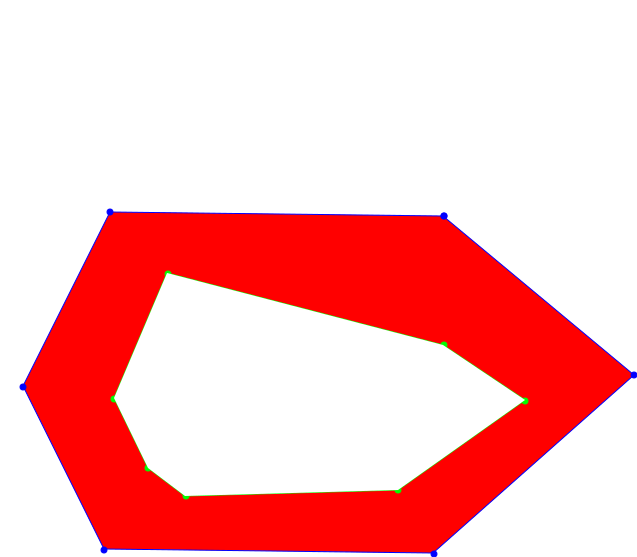
\includegraphics[scale=.6]{SymDiff.eps}
	\caption[Die symmetrische Differenz zweier Polygone]{Die symetriche Differenz der beiden Polygone aus dem Schaubild \ref{fig:HausdorffAbstand} ist der Flächeninhalt der roten Fläche.}
	\label{fig:SymDiffBild}
\end{figure}

In \cite{AFRW} wird vorgeschlagen den Fl"acheninhalt der symmetrischen Differenz als Abstands-Ma"s zweier konvexer Polygone zu benutzen. Die Symmetrische Differenz von zwei kompakten Teilmengen $A$ und $B$ des $\mathbb{R}^2 $ ist definiert als:
\[A\bigtriangleup B:=(A\setminus B)\cup(B\setminus A).\]
Wenn $A(\cdot)$ der Fl"acheninhalt ist, so bildet $\delta_S$ den Abstand nach der symmetrischen Differenz:
\[\delta_S:=A(A \bigtriangleup B).\]
in \cite{TG} schlagen die Autoren vor, die Überlappung $A\cap B$ als Maß für die Qualität eines Matchings zu benutzen. Wegen:
$$|A\bigtriangleup B|+|A\cap B|=|A\cup B|$$
ist klar, dass ein Match, dass die symmetrische Differenz minimiert,zu dem selben Ergebniss kommen wird, wie ein Match, dass die Überlappung maximiert.

In \cite{AFRW} wurde beschrieben, dass das Verhalten der symmetrischen Differenz relativ ,,gutmütig'' im Bezug auf gestörte Daten sei. Die Zeichnung \ref{fig:VergleichMetrik} erläutert diesen Zusammenhang. Die beiden Polygone sehen den Polygonen aus den Bildern \ref{fig:HausdorffAbstand} und \ref{fig:SymDiffBild} recht ähnlich, nur zwei Punke sind jedem Polygon ergäntzt worden. Dennoch ist der Hausdorf-Abstand um 100\% gestiegen, die Fläche der symmetrischen Differenz hingegen nur etwa um 8\%.

\begin{figure}
	\centering
	\includegraphics[scale=.6]{Metrikengestoert.eps}
	\caption{Hausdorff-Abstand und symmetrische Differenz im Vergleich}
	\label{fig:VergleichMetrik}
\end{figure}


\subsection{\index{Steinerpunkt!Definition}Der Steinerpunkt}\label{Steinerpunkt}

In \cite{Sch} wird der Steinerpunkt beschrieben "`als Schwerpunkt der Massenverteilung, die bei einem konvexen Polygon duch Belegung der Ecken mit den "au"seren Winkeln als Massen [...] gegeben ist"'. Folglich kann der Steiner-Punkt eines konvexen Polygones $P$, das aus den $n$ Eckpunkten $v_i$ besteht, berechnet werden ($\alpha_i$ ist hierbei der Innenwinkel von $v_i$) durch:
\[p_2(P)=\sum^n_{i=1}v_i (\pi-\alpha_i).\]
In der Zeichnung \ref{fig:Referenzpunkte} ist der Steienerpunkt grün eingezeichnet.


\subsection{\index{Schwerpunkt!Definition}Der Schwerpunkt}\label{Schwerp}

Der Schwerpunkt eines Polygones ist der Schwerpunkt der Massenverteilung, die entsteht, wenn man allen Eckpunkten die selbe Masse zuordnet. Er berechnet sich f"ur ein Polygon $P$ mit $n$ Eckpunkten $v_i$:
\[p_0(P)=\sum^n_{i=1}v_i \frac{1}{n}.\]
In der Zeichnung \ref{fig:Referenzpunkte} ist der Schwerpunkt mit roter Farbe markiert. 

Vergleicht man die beiden Referenzpunkte, so kann man sehen, dass der Schwerpunkt etwas ,,träger'' auf Punkte reagiert, die sich stark von den anderen unterscheiden (in dem dargestellten Beispiel der Punkt ganz rechts). In einem regelmäßigen n-Eck stimmen entsprechend beide Referenzpunkte überein. Vergleicht man dieses Verhalten der Referenzpunkt mit dem Verhalten der Normen für gestörte Werte (siehe Abbildung \ref{fig:VergleichMetrik}), so erscheint der Zusammenhang vom ,,empfindlicheren'' Hausdorff-Abstand und dem  Steinerpunkt, sowie der Zusammenhang zwischen den beiden ,,Gutmütigeren'' plausibel.

\begin{figure}
	\centering
	\includegraphics[scale=.8]{Referenzpunkte.eps}
	\caption[Vergleich beider Referenzpunkte]{Hier kann man beide Referenzpunkte im Vergleich sehen (der Schwerpunkt der Massenverteilung ist rot, der Steinerpunkt grün) }
	\label{fig:Referenzpunkte}
\end{figure}



\chapter[Eigene "Uberlegungen und die Implementierung \anmerkung{30 Seiten }]{Eigene "Uberlegungen und die Implementierung der resultierenden L"osung
\normalsize{Die Java-Applikation, Die Secondo Algebra, Experimante mit Regionen \anmerkung{30-40 Seiten }}
}
\minitoc
\newpage
\section{Vor"uberlegungen \anmerkung{7 Seiten}}
\anmerkung{Hier beschreibe ich welche Gedanken ich mir zum Theme Matching gemacht habe, und welche davon ich verwirklicht habe. Ausserdem bewerte ich die Vorschl"age aus der Literatur, die ich oben bereits erw"ahnt habe.}
\subsection{Bewertung der Vorschl"age von Herr  T\o{}ssebro}
\begin{enumerate}
\item Position of centroid

In dem Paper wurde diese M"oglichkeit nicht weiter betrachtet, da die Autoren davon ausgehen, dass ein Referenzpunkt, der auch au"serhalb des Polygons liegen kann nicht zu guten Matchings f"uhren kann. Hierzu muss angemerkt werden, dass im Rahmen der vorliegenden Arbeit das Matching auf Ebene des ConvexHullTrees durchgef"uhrt wird, und lediglich mit konvexen H"ullen von Polygone gearbeitet wird. Der Schwerpunkt einer konvexen H"ulle liegt nat"urlich aber wieder innerhalb dieser (wenngleich nicht zwangsl"aufig auch innerhalb des repr"asentierten Polygons). Au"serdem erscheint es plausibel, dass ein Referenzpunkt-Verfahren seine St"arke gerade dort haben wird, wo die "Uberlappungsalgorithmen ihre Schw"achen haben (bei sich schnell bewegenden, kleinen Objekten).

Der Vorschlag, "`N"achste Nachbarn"' zu benutzen, hat den Nachteil, dass man so nur 1:1 Matches finden kann. Im Rahmen der vorliegenden Arbeit wurde stattdessen Schwellwert-Verfahren gew"ahlt, in dem zu einem Element der einen Seite, alle Elemente der Anderen gematcht werden, deren Schwerpunkte weniger als "`Schwellwert"' entfernt sind. 

\item Fixend threshold (set of cycles)

Das Verfahren wurde analog zur Beschreibung Erlend T\o{}ssebros "ubernommen und implementiert. 

\item Maximize Overlap (set of cycles)

Dieses Verfahren k"onnte interesannt sein, ist aber noch nicht implementiert.

\item Matching mit dem Steiner-Punkt

In dem Aufsatz \cite{AAR} wurde das Matching mit dem Steiner-Punkt als Referenzpunkt durchgef"uhrt. Auch wenn die Grundausrichtung dieser Arbeit von meiner verschieden ist, so ist es doch m"oglicherweise interessant, diese Spur weiterzuverfolgen. Zu dem eigentlichen Ablauf des Matchings gilt dasselbe, wie f"ur das Schwerpunktverfahren.
\end{enumerate}

\subsection{Matching mit Referenzpunkten}

Unter der Annahme, dass es möglich ist zu jedem Polygon, das gematcht wird ein Referenzpunkt zuberechnen, kann ein Feld aufgebaut werden, in dem zu jeder Kombination von Cycles die Entfernung der Referenzpunkte eingetragen werden kann. Wird dieses Feld aufsteigend nach den Entfernungen geordnet, steht zu erwarten,
dass es zwischen den erwünschten und den unerwünschten Matches einen Sprung in dem Graphen geben wird. 

Nehmen wir also an, wir haben eine M"oglichkeit, zu jedem Polygon, das wir matchen wollen einen Referenzpunkt zu berechnen. Dann k"onnen wir ein Feld aufbauen, in dem zu jeder Kombination von Cycles die Entfernung der Referenzpunkte eingetragen werden. Ordnen wir dieses Feld aufsteigend nach den Entfernungen, so steht zu erwarten, dass es zwischen den erw"unschten und den unerw"unschten Matches einen Sprung in dem Graphen geben wird. Diesen Sprung m"u"ste man mit geeigneten statistischen Verfahren finden k"onnen. 

Nachteilig an diesem Verfahren ist, dass die Laufzeit dieses Verfahrens hoch ist. Haben wir auf den beiden Seiten des Matchings $n$ beziehungsweise $m$ Referenzpunkte, so ist hat das resultierende Feld die Dimension $n\times m$. Dieses Feld kann man in $O(n\times m)$aufbauen. Zum Sortieren des Feldes braucht man dann $O((n\times m)\log(n\times m))$. Also ist dises Verfahren mindestens vom Typ $O((n\times m)\log(n\times m))$ (je nach dem verwendeten statistischen Verfahren k"onnte die Laufzeit sogar schlechter sein).

Wegen dieser schlechten Laufzeit, und weil ich noch kein geeignetes Verfahren gefunden habe, verwende ich das wesentlich einfachere Schwellwertverfahren, dass man formulieren kann: Matche zwei Cycle, wenn der Abstand ihrer Referenzpunkte kleiner als der Schwellwert ist. 

Die Laufzeit dieses Verfahrens ist wesentlich besser. Ich berechne zu jeder der $m\times n$ verschiedenen  Referenzpunkte den Abstand (in konstanter Zeit) und vergleiche diesen mit dem Schwellwert. Also ist die Laufzeit$O(n\times n)$.

Aufgrund der Verschiedenheit der m"oglichen Daten ist ein solcher absoluter Schwellwert $t_{abs}$ nat"urlich nicht handhabbar, so dass die Matchingfunktion mit einem relativen Schwellwert $t_{rel}$ (in \%) arbeiten muss. Aus Diesem wird dann intern ein absoluter Schwellwert berechnet, der dann wie oben verwendet wird. Man berechnent $t_{abs}$, indem man $t_{rel}$ mit dem gr"o"sten Abstand multipliziert, den die beiden Regionen voneinander haben. Leider ben"otigt man f"ur die Berechnung dieses Wertes $O(n\times m)$. Praktisch verwende ich desshalb einen Algorithmus, der mir in $O((n+m)\log{n+m})$ einen sehr "ahnlich Wert berechnet. Siehe hierzu: "`Spezielle Algorithmen"'.
\subsection{Beseitigung von 1:n Matches}

Falls es ein 1:n Matching gibt, dann muss diese aufgel"ost werden. Hierbei existieren 2 M"oglichkeiten:
\begin{itemize}
\item Alle $n$ Targets sind Kinder einer einzigen ConvexHullTreeNode

Dieser Fall ist der einfachere, seine Behandlung wurde schon von Herrn T\o{}ssebro beschrieben. Kurz gesagt geht es darum, die konvexe H"ulle aller Targets zu bilden, und das Matching von den $n$ Targets auf diese neue H"ulle umzuleiten.

\item Alle n Targets haben unterschiedliche V"ater

In diesem Fall kommen wir mit der Vereinigung der Targets, wie oben beschrieben, nicht weiter, also m"ussen wir versuchen, den Source aufzuteilen. Hiebei ist zu beachten:
\begin{itemize}
\item Eine ConvexHullTreeNode kann man nur an Eckpunkten, oder an Punkten auf Linien teilen, die keine Kinder haben, da man sonst den ConvexHullTree zerst"oren w"urde.

\item Eine ConvexHullTreeNode kann man nur an zwei Punkten teilen, wenn das beschriebene Polygon auch nur in zwei Teile zerf"allt.
\item Zerteilt man ein Face, so sollte man dabei kein Hole zerteilen. Falls sich das nicht verhindern l"asst, so zerf"allt das Loch in zwei Konkavit"aten, was eine Neuberechnung der entsprechenden Matchings zu Folge hat.

\item Die Zerteilung der Source-Komponente sollte die Lage und das Verh"altnis der Fl"acheninhalte der Target-Komponenten weitestgehend wiederspiegeln.

\end{itemize} 
\end{itemize} 
\subsection{Beseitigung von "`gedrehten Konkavit"aten"'}
In manchen F"allen versagt das in \cite{TG} genannte Verfahren, um aus Matchings Moving-Regions zu erzeugen. Dieses, in Kapitel "`6 Interpolating between two arbitray polygones"' beschriebene Verfahren setzt voraus, dass die beiden gematchten Kinderpolygone ein gemeinsames, aus zwei Dreiecken zusammengesetztes Trapez in der Aussenh"ulle der beider Vaterpolygone besitzen. 

Dies ist zum Biespiel dann nicht der Fall, wenn wir uns als Quellpolygon ein "`U"', und als Zielpolygon ein um 90$\degree$ gedrehtes "`U"' vorstellen. Auch wenn die Konkativit"aten richtig zueinander gematcht sind, versagt das bekannte Verfahren.

Die, das Matching abschlie"sende, Funktion kann solche F"alle erkenne, indem es die Winkel betrachtet, die die gemeinsame Kante von Kind und Vater, sowie die beiden Nachbarkanten des Vates, mit der x-Achse haben. Ist der Winkel der gemeinsamen Kante auf der einen Seite nicht im  Intervall der Winkel der Nachbarkanten der anderen Seite, so liegt der Fal vor, dass das Verfahren nicht funktioniert.

Wenn ein solcher Fall erkannt wird, so gibt es zwei M"oglichkeiten zu reagieren:
\begin{itemize}
\item Beide Konkativit"aten werden gegen $null$ gematcht

In diesem Fall sehen wir, wie die Konkativit"at auf der einen Seite verschwindet, und zeitgleich auf der anderen Seite eine Neue entsteht. Obwohl dieses Verfahren das deutlich Einfachere ist, sieht das Resultat recht gut aus.

\item Die beiden Konkativit"aten werden zu L"ochern umgewandelt

In diesem Fall werden beide Konkavit"aten in L"ocher verwandelt, die dann zueinander gematcht werden. In dem Resultat w"urde man also sehen, wie sich die Konkativit"at von der einen Seite abl"ost, und zu der anderen Seite wandert. M"oglicherweise sieht dieses Verfahren nat"urlicher aus, man muss sich aber noch "uberlegen, was passiert, wenn der Weg zwischen den beiden Positionen nicht "`frei"' ist (etwa weil sich hier ein weiteres Loch oder eine Konkativit"at befindet).

\end{itemize}


\subsection{Erstellung eines Matchings aus mehreren Anderen}

Wenn man die bereits ausprobierten Matchings betrachtet, so stellt man fest, dass das Overlapping-Match besser auf Vereinigungen und Aufsplitterungen von Cycles reagiert, und dass das Schwerpunkt-Verfahren besser auf kleine und schnelle Cycles abgestimmt ist. 

Es scheint also ein verfolgenswerter Ansatz zu sein, beide Matches (und vielleicht noch andere, etwa Overlapping mit mehreren Schwellwerten), zu berechnen, und aus diesen das beste Matching zu bestimmen. 

Um die G"ute eines gegebenen Matchings zu bestimmen, habe ich folgende Verfahren erdacht. Damit die verschiedenen Bewertungen vergleichbar sind, habe ich diese auf 1 normiert.
\begin{itemize}
\item Die Overlapp-Bewertung: 

Ist der Duchschnitt der "Uberlappungen gro"s, so ist das gut.

Dieses Bewertungsverfahren korespondiert zwar direkt mit dem Overlaping-Match, da es aber in \cite{AFRW} verwendet wird, benutze ich dieses Verfahren. Die Berechnung l"auft so:

$$r_O=\frac{\sum_{m\in M} \frac{A_{overlap}}{A_{source}+A_{target}}}{|M|}$$

\item Die Schwerpunkt-Bewertung:

Ist die durchschnittliche Entfernung der zueinander gematchten Schwerpunkte gro"s, so ist das schlecht.

Da dieses Verfahren direckt mit dem Schwerpunkt-Match korespondiert, und ausserdem nach \cite{AFRW} nicht zu erwarten steht, dass dieses Verfahren eine deutlich andere Werte als die Overlap-Bewertung liefert, verfolge ich dieses nicht weiter.

\item Die Summen-Norm:

Sind die zueinander gematchten Fl"achen etwa gleich gro"s, so ist das gut. 

Es steht zu erwarten, dass zueinander geh"orige F"achen etwa gleich gross sind. Auch wenn sich eine Fl"ache in mehrere andere teilt, wird die Summe der Fl"acheninhalte in etwa so gro"s sein, wie der Fl"acheninhalt der Ursprungsfl"ache. Zur Normierung teile ich den Kleineren durch den gr"o"seren Fl"acheninhalt, und bekomme somit die Abweichung in Prozent. Die Berechnung l"auft so:

$$A_{target}=\sum_{t\in Target}A_t$$
$$r_A=\frac {\sum_{m\in M}\frac{\min{A_{source},A_{target}}}{\max{A_{source},A_{target}}}}{|M|}$$

\item Die \index{Hausdorff-Norm}Hausdorff-Norm:

In \cite{AAR} wird die,  oben bereits eingef"uhrte, Hausdorff-Norm benutzt, um Matchings zu bewerten. 

Bei der Implementierung dieser Norm stellt sich die Frage der Normierung. Mangels Alternative habe ich mich dazu entschlossen, alle einzelnen Hausdorff--Abst"ande duch den Duchmesser $d$ der Ausgangsregionen zu teilen.  Durchmesser bezeichne hierbei den Gr"o"sten Abstand, den zwei Punkte zueinander haben. Dieses Vorgehen bedeutet aber leider, dass die Abst"ande von kleinen Konkavit"aten relativ wenig in die Gesamtbewertung eingehen. Die Berechnung lautet:

$$r_H=\frac{\sum_{m\in M}\delta_H(m)}{|M|\times d}$$


\item Die Linear-Norm

Bei der Implementierung der obigen Verfahren zeigte sich, dass die Verfahren eine Tendenz zu "ubertriebenen Zersplitterungen aufweisen. Unter der Pr"amisse, dass dies in den allermeisten F"allen eher selten der Fall ist, f"urte ich diesen Bewertungsfaktor ein, um dieses Verhalten abzuschw"achen.

F"uhrt das Matching zu einer geringen Anzahl an Zersplitterungen, so ist das gut.

Die Berechnung l"auft so:




$$L(m)=
\begin{cases}
	\frac{1}{2} & \text{falls }|targets|=0\\
	\frac{1}{|targets|} & \text{sonst}
    \end{cases}
$$

$$r_L=\frac{\sum_{m\in M}L(m)}{|M|}$$

\item Die Struktur-Norm:

Stimmen die aufeinander gematchten Cycles strukturell weit "uberein, so ist das gut (eventuell kann man hier die Struktur der jeweiligen ConvexHullTrees heranziehen).

Diese Norm finde ich nach wie vor interesant, habe sie aber noch nicht weiter verfolgt. Nach der Betrachtung der Ergebnisse aus den anderen Normen, scheint eine weitere Verfolgung auch nicht notwendig. Zur Struktur der ConvexHullTrees ist zu sagen, dass in \cite{TG} der Umstand beschrieben ist , das "ahnliche Polygone teilweise recht unterschiedliche ConvexHullTree-Repr"asentationen aufweisen k"onnen, was eine solche Bewertung nat"urlich negativ beweinflussen kann\footnote{Dieses ist aber weniger schlimm als es klingt, Herr T\o{}ssebro macht in diesem Artikel plausiebel, dass dieses Problem eher ein Problem von kleinen, k"unstlichen Testdatens"atzen als von realen Daten ist}.


\end{itemize} 

Wie man am Beispiel der Summen-Norm sehen kann, gibt es mehr M"oglichkeiten zu bewerten, als es effiziente Matchings gibt. Das Summen-Matching, das lauten k"onnte: "`Matche ein Cycle mit  einer Menge von Anderen, wenn die Summe der Fl"acheninhalte fast gleich ist zu dem Fl"acheninhalt des einen Cycles"', entspricht dem Rucksack-Problem und ist daher nicht effizient l"osbar. Die Bewertung, wie gut ein gegebenes Matching ist, sollte mit diesem Verfahren aber effizient m"oglich sein.

\section{Gemeinsame Grundlagen \anmerkung{20 Seiten}}
\anmerkung{Hier beschreibe ich ausf"uhrlicher die gemeinsame Grundlage der beiden Implementierungen, einschlie"slich einer Beschreibng der verwendeten Klassen.}
\subsection{Beschreibung der Klassen}
\subsubsection{RegionTreeNode}

Dieses Interface dient dazu, Region, Faces und ConvexHullTreeNodes gleichbehandeln zu k"onnen. Implementiert sind nur hashCode und equals, zum Auffinden von SingleMatches in HashSets.

\subsubsection{\index{SingleMatch}SingleMatch}
Diese Klasse repr"asentiert eine einzelnes Teilmatch.  Es enth"alt eine Source-Kom"-ponente und ein Feld von Target-Komponenten. Alle Komponenten sind RegionTreeNodes.
Die wichtigsten Methoden sind:

\begin{itemize}
\item Der Konstruktor

Der Konstruktor legt ein SingleMatch zwischen den Komponenten Source und Target an. Es kann nur ein einziges Target "ubergeben werden, weitere m"ussen mit addTarget hinzugef"ugt werden.



\item addTarget

Diese Methode f"ugt eine weitere Target-Komponente hinzu.

\item getNrTargets

Diese Methode liefert die Anzahl der Targets.

\item getTargetAt

Diese Methode liefert das Target mit dem "ubergebenen Index zur"uck.

\item removeTargets

Diese Methode l"oscht alle Targets dieses SingleMatches.

\item hashCode

Liefert den Hashwert des Matches.

\item equals

"Uberpr"uft zwei Komponenten auf Gleichheit.

\end{itemize}

Die beiden letzten Methoden dienen dazu, SingleMatches in einem HashSet ablegen zu k"onnen, wobei nur die source-Komponente f"ur das Auffinden des Matches herangezogen wird.

\subsubsection{\index{Match!Klasse}Die abstrakte Klasse Match}
Diese Klasse stellt die wesentlichen Mechanismen zur Verf"ugung, um einfach Matches programmieren zu k"onnen. Es enth"alt die Eigenschaften:
\begin{itemize}
\item source

Die Region zum Eingangszeitpunkt.

\item target

Die Region zum Ausgangszeitpunkt.

\item maps

Ein Hashtable, in dem die einzelenen Teilmatches abgelegt werden. Der Schl"ussel, um auf die Elemente dieses Tables zugreifen zu k"onnen ist die Quell-Komponente vom Typ RegionTreeNode.

\item name

Der Name des Matches.

\item description

Eine Beschreibung, wie das Matching funktioniert.
\end{itemize} 

Diese Klasse verf"ugt "uber einige Methoden, die wichtigen davon  sind:

\begin{itemize}

\item Der Konstruktor

Setzt Name, Beschreibung, Source und Target auf die angegebenen Werte und initialisiert ein leeres Hashtable.

\item addMatch

Diese Methode f"ugt ein neues Match von Source nach Target ein. Sollte es noch kein Match von Source aus geben, so legt er ein neues Match an, und erweitert anderenfalls das Vorhandene.

\item getMatches

Diese Methode liefert ein Feld mit allen Targets, die von Source aus gematcht sind.

\item getTargetChildren

Diese Methode liefert alle Kinder der Targets als Feld aus. Falls ein Target ein ConvexHullTreeNode ist, dann finden sich im R"uckgabefeld alle seine Kinder  wieder, falls Target ein Face ist, dann werden alle Holes und die Kinder des Cycles zur"uckgegeben. Diese Sonderbehandlung des Faces ist n"otig, da man ein Face mit seinem Cycle identifizieren kann, und die L"ocher also quasi Kinder des Cycles sind.

\item fertig

Die Erzeugung von Dreiecken bzw. MovingLines mit der Klasse mLineRep funktioniert nur, falls nur 1:1 Matchings vorkommen. Nach der Erzeugung des Matchings ist das im Allgemeinen nicht gew"ahrleistet, desshalb muss man am Ende der Erzeugung diese Methode aufrufen, die sich darum k"ummert. Auch die Beseitigung von zu stark gedrehten Konkativit"aten findet hier statt. N"aheres zum Ablauf dieser Funktion folgt weiter unten.

\item Die Bewertungsfunktionen

In dieser Klasse sind auch einige der Bewertungsverfahren implementiert, die in dem allgemeinen Matching-Teil beschrieben sind. Im einzelnen sind dass:
\begin{itemize}
\item Das Area-Rating
\item Das Hausdorff-Rating
\item Das Linear-Rating
\item Das Overlap-Rating
\end{itemize}

\end{itemize}

\subsection{Beschreibung von verwendeten Algorithmen}
In disem Abschnitt werde ich Algorithmen vorstellen, die entweder sehr zentral f"ur die L"osung des Interpolationsproblems sind, oder Algorithmen, die keine Standard-Algorithemen sind. Diese Algorithmen musste ich also selbst entwickeln.

\subsubsection{Rotaring Pane}
\begin{algorithm}
		\SetKwFunction{fMI}{finde\_passenden\_Index}
	\caption{Rotaring Pane Allgorithmus, um aus zwei konvexen H"ullen moving segments zu erstellen}
	\Ein{KH"ulle1 und KH"ulle2, zwei konvexe H"ullenb"aume}
	\Ergebnis{Eine Menge von moving segments, die die Interpolation der beiden Polygone darstellt}
	\Begin{
		Bestimme $KH1$ und $KH2$ die konvexen H"ullen der Polygone als Feld von LineWAs\;
		Berechne die Winkel in jedem Eckpunkt von $KH1$ und $KH2$\;
		Sortiere $KH1$ und $KH2$ aufsteigend nach diesen Winkeln\;
		$j:=0$\;
		\Fuer{$i<KH1.l"ange$}{
			$j:=\fMI{KH2, j, KH1[i].winkel, \text{false}}$\;
			F"uge das moving segment:$(KH1[i],KH1[i+1],KH2[j]$ dem Ergebnis-Feld hinzu\;
		}			
		$j:=0$\;
		\Fuer{$i<KH2.l"ange$}{
			$j:=\fMI{KH1, j, KH2[i].winkel,\text{true}}$\;
			F"uge das moving segment:$(KH2[i],KH2[i+1],KH[j]$ dem Ergebnis-Feld hinzu\;
		}			
	}
\end{algorithm}

\begin{function}
	\caption{finde\_passenden\_Index(Polygon, Startindex, Winkel, Gleiche\_Winkel)}
	
	\Ein{\begin{tabular}{ll}
		Polygon: &Das zu durchsuchende konvexe Polygon als Feld\\
 			&von LineWAs\\
		Startindex: &Der Index, an dem die Suche beginnen\\
 				&soll\\
		Winkel: &Der Winkel, zu dem der passende Index gesucht\\
 			&wird\\
		Gleiche\_Winkel: &Dieser boolsche Parameter gibt an, \\
				&wie mit parallelen Kanten verfahren werden soll
	     \end{tabular}
	}
	\BlankLine
	\Ergebnis{Der Index des Punktes, an dem die Linie anf"angt, mit der die Ecke mit dem "ubergebenen Winkel gematched wird}
	\Begin{	
        	\uWenn {$Winkel<Polygon[0].Winkel$}	{
        		Gebe den Index 0 zur"uck\;
		}
        	\uWenn{$Polygon[0].Winkel=Winkel$ und $Gleiche\_Winkel$}{
        			Gebe den Index 0 zur"uck\;
		}        
        	\Wenn{$Winkel>Polygon[letzer\_Index].Winkel$}{
        		Gebe den Index 0 zur"uck\;
		}
	
        	\Solange{Nicht $(Polygon[j].Winkel\geq Winkel$ und $Polygon[j-1].Winkel\leq Winkel)$}{
        		\uWenn{$(j\neq0$ und $Winkel<Polygon[j-1].Winkel$}{
        			$j:=j-1$\;
			}	
 	           	\Sonst{
				\Wenn{$Polygon[0].Winkel\neq Winkel$}{
		                 	$j:=j+1$\;
				}
			}
		}
		\Wenn{$Polygon[j].Winkel=Winkel$ und $Gleiche\_Winkel$}{
	        	$j:=j+1$\;
		}
		Gebe den Index $j$ zur"uck\;
	}		
\end{function}
\clearpage
\subsubsection{Zerlegung von einfachen Polygonen in konvexe Polygone}
\begin{algorithm}
	\SetKwFunction{gCV}{liefere\_konvexe\_Ecken}
	\SetKwFunction{iSA}{ist\_teilbar}
	\caption{Zerlegung von einfachen Polygonen in konvexe Polygone}
	\Ein{Eine Menge $Polygone$ von einfachen Polygonen, repr"asentiert durch geordnete Punktlisten}
	\Ergebnis{Die Menge $Polygone$ besteht nur noch aus konvexen Polygonen}
	\Begin{
		$aktuell:=0$\;
		$konvexe\_Ecken=\emptyset$\;
		\Wiederh{$|konvexe\_Ecken|=0$ und $aktuell=|Polygone|$}{
            		$aktuelles\_Polygon=Polygone[aktuell]$\;
			$konvexe\_Ecken=aktuelles\_Polygon.\gCV{}$\;
			\uWenn{$|konvexe\_Ecken|>0$}{
				\Wenn{$|konvexe\_Ecken|>1$}{
					\Fuer{$i<|konvexe\_Ecken|$}{
						\Fuer{$j:=i+1$ \KwTo $j<|konvexe\_Ecken|$}{
							\Wenn{$aktuelles\_Polygon.\iSA{konvexe\_Ecken[i],konvexe\_Ecken[j]}$}{
								Teile $aktuelles\_Polygon$ an den Ecken $konvexe\_Ecken[i]$ und $konvexe\_Ecken[j]$\;
								Ersetzt $aktuelles\_Polygon$ in $Polygone$ durch die beiden neuen Polygone\;
								Durchlaufe alle Scheifen von neuem\;
							}
						}
					}
				}
                		$Index1:=konvexe\_Ecken[0]$\;
				$Index2:=Index1+\frac{|aktuelles\_Polygon|}{2}$\;
				\Fuer{$i<|aktuelles\_Polygon|$}{
					$split\_Index=Index2+\frac{(-1)^i i}{2}$\;
		                    	\Wenn{$aktuelles\_Polygon.\iSA{Index1,split\_Index}$}{
		                    	Teile $aktuelles\_Polygon$ an den Ecken $Index1$ und $split\_Index$\;
								Ersetzt $aktuelles\_Polygon$ in $Polygone$ durch die beiden neuen Polygone\;
					}
				}
			}
			\Sonst{
				$aktuell:=aktuell+1$\;
			}

		}
	}
\end{algorithm}
\clearpage
\subsubsection{Aufbau eines ConvexHullTrees}
Der Algorithmus zum Aufbau eines ConvexHullTrees wurde in \cite{TG} bereits erl"autert. Da dieser aber von zentraler Bedeutung zur L"osung des Problems ist, bespreche ich den Algorithmus an dieser Stelle noch einmal.

Als Beispiel dient mir ein Polygon aus der GERMANY-Datenbank. Bei diesem Polygon handelt es sich um die Gemeinde Sandershausen, die als Enklave zu dem Stadtkreis Kassel geh"ort. Abbildung \ref{fig:Sanders} zeigt dieses Polygon in dem dazugeh"origen Luftbild, dass ich aus der Applikation Google-Earth entnommen habe. 

Der erste Schritt, bei der Erzeugung eines ConvexHullTree-Kontens, ist die Ereugung der konvexen H"ulle des Polygons. In den Abbildungen \ref{fig:sand2} und \ref{fig:sanders3} ist diese in Rotbraun eingezeichnet. Der Allgorithmus, der zur Erzeugung der H"ulle benutzt wird ist der \index{Graham Scan}Graham Scan Algorithmus, der zu den Standard-Allgorithem zu z"ahlen ist. In \cite{G72} wurde dieser Algorithmus das erste Mal beschrieben. Eine gute Beschreibung finden Sie \anmerkung{hier Literaturstelle einf"ugen}.

Im Anschu"s daran wird das Ausgangspolygon nach zusammenh"angenden Linienz"ugen durchsucht, die nicht in der konvexen H"ulle enthalten sind. Diese Suche wird mittels eines parallelen Durchlaufs duch beide Linienz"uge realisiert.

Schlie"slich wird diser Algorithmus rekursiv f"ur alle diese Linienz"uge aufgerufen und die Ergebnisse werden an die entsprechenden Stellen in den Vaterknoten eingeh"angt.

\begin{figure}
	\centering
	\includegraphics[height=5cm]{Sandershausen.eps}
	\caption{Die Gemeinde Sandershausen als Beispiel eines ConvexHullTrees}
	\label{fig:Sanders}
\end{figure}
\begin{figure}
	\centering
	\includegraphics[width=5cm]{Sandershausen2.eps}
	\caption{Ausschnitt von Sandershausen mit den Nodes der Level 0-1}
	\label{fig:sand2}
\end{figure}
\begin{figure}
	\centering
	\includegraphics[width=5cm]{Sandershausen3.eps}
	\caption{Ausschnitt von Sandershausen mit dem kompletten ConvexHullTree}
	\label{fig:sanders3}
\end{figure}

\begin{algorithm}

\SetKwFunction{cH}{berechne\_konvexe\_H"ulle}
	\caption{Erzeuge einen konvexen H"ullenbaum aus einem Polygon}
	\Ein{\begin{tabular}{ll}
		Polygon: &Ein Polygon,rep"asentiert duch eine geordnete Liste von \\
			&Eckpunkten\\
		Ebene:	&Die Ebene des zu Erzeugenden Elementes\\
		ist\_Loch: &Ein boolscher Parameter der angibt, ob das neue Element \\
			&zu einem Loch geh"ort\\
		Vater:	&Das Vaterelement des Neuen\\
		\end{tabular}
	}
	\BlankLine
	\Ergebnis{Ein konvexer H"ullenbaum, der das "ubergebene Poygon beschreibt}
	\Begin{
	
%         LineWA[] tmplist, convhull, childlist;
	Setze die Klassen-Variabeleln $ist\_Loch$ und $Vater$\;

%         int node;
%         int index1, index2, length, lastindex, noiterations;
%         int indexll1, indexll2;
%         this.linelist = new Vector();
%         smallesty = Integer.MAX_VALUE;
%         smallestx = Integer.MAX_VALUE;
%         smallestpoint = -1;       
	$konvexeH"ulle:=\cH(Polygon)$\;
%         // Find where the first node in linelist is in the convex hull
%         // (Or the earliest possible if the first node is not on the hull)
%         // This is to preserve the order in the linelist in the ordering of
%         // points in the convex hull tree node.
	$startindex:=0$\;
	$endindex:=konvexeH"ulle.L"ange$\;
	Finde den Index, in der konvexen H"ulle, der dem niedrigsten Index in dem Polygon entspricht, und speichere Ihn in $startindex$\;
	Finde den Index, in der konvexen H"ulle, der dem h"ochsten Index in dem Polygon entspricht, und speichere Ihn in $endindex$\;
         %for (int a=0;a<linelist.length;a++)
% {
%             index1 = TriRepUtil.indexOf(convhull, linelist[a]);
%             if (index1 != -1) break;
% }
%         for (int a=linelist.length-1;a>=0;a--)
% {
%             lastindex = TriRepUtil.indexOf(convhull, linelist[a]);
%             if (lastindex != -1) break;
% }
	\uWenn{$startindex<endindex$}{
		\Fuer{$i:=startindex$ \KwTo $i\leq endindex$}{	
			Speichere $konvexeH"ulle[i]$ in der linelist des neuen Konten\;
		}
	}
	\Sonst{
		
        	\Fuer{$i:=index1$ \KwTo $konvexeH"ulle.L"ange$}
		{
			Speichere $konvexeH"ulle[i]$ in der linelist des neuen Konten\;
		}
		\Fuer{$i:=0$ \KwTo $endindex$}
		{
			Speichere $konvexeH"ulle[i]$ in der linelist des neuen Konten\;
		}
	}
%         // Check lines in convex hull with lines in line list. Whenever two points
%         // which are neighbours in the convex hull are not neighbours in the line
%         // list, create a child node from the points between them.
%         
%         noiterations = numberOfLines();
%         index1 = 0;
%         indexll1 = 0;
%         while (!(linelist[indexll1].equals(getLine(index1))))
% {
%             indexll1++;
% }
	\Fuer{$i<konvexeH"ulle.L"ange$}
	{
%             index2 = index1+1;
%             indexll2 = indexll1+1;
%             while (!(linelist[indexll2 % linelist.length].equals(getLine(index2 % noiterations))))
% {
%                 indexll2++;
% }
%             
%             if ((indexll2 != indexll1+1) && ((level == 0) ||
%                     ((indexll2 != linelist.length) && (indexll1 != linelist.length-1)))
%                     && (indexll2 != indexll1-1))
% {
%                 // create child node
%                 length = indexll2-indexll1+1;
%                 childlist = new LineWA[length];
%                 for (int b=0;b<length;b++)
% {
%                     if ((b+indexll1) < linelist.length)
% {
%                         childlist[length-b-1] = linelist[b+indexll1];
% }
%                     else
% {
%                         childlist[length-b-1] = linelist[b+indexll1-linelist.length];
% }
% }
%                 insertChild(index1, new ConvexHullTreeNode(childlist, level+1,this.isHole,this));
% }
%             index1 = index2;
%             indexll1 = indexll2;
	}
}
 \end{algorithm}
\clearpage
\subsubsection{Bestimmung der maximalen Distanz mehrerer Polygone}
\begin{algorithm}
	\SetKwFunction{gLDFP}{l"angste\_Entfernung\_von\_Punkt}
	\SetKwFunction{dist}{Quadrat\_der\_Entfernung}
	\caption{Bestimmung der maximalen Distanz mehrerer Polygone}
	\Ein{Mehrere Polygone repr"asentiert duch ihre Punktlisten}
	\Aus{Der maximale Abstand von zwei Punkten}
	\Begin{
		Bilde eine gemeinsame Punktliste durch konkatenieren der Eingangslisten\;
		Bilde $CH$ die konvexe H"ulle der Eingangsdaten\;
		$i:=0$\; 
		$tmpdist:=0$\;
		$pos:=frac{CH.length}{2}$\;
		\Fuer{$i<CH.length$}{
			$pos:=\gLDFP{CH[i],CH,pos}$\;
			$distxy:=\dist{CH[i],CH[pos]}$\;
		        \Wenn{$distxy>tmpdist$}
			{			
			           $tmpdist:=distxy$\;
			}			
		}    
		Das Ergebnis ist $\sqrt{tmpdist}$\;
	}
\end{algorithm}

\begin{function}
	\SetKwFunction{dist}{Quadrat\_der\_Entfernung}
	\SetKwFunction{gLDFP}{l"angste\_Entfernung\_von\_Punkt}
	\caption{l"angste\_Entfernung\_von\_Punkt(Punkt, Polygon, Startindex)}
	\Ein{\begin{tabular}{ll}
Punkt: &Der Punkt, zu dem der Abstand gemessen wird,\\
	     Polygon: &Das Polygon, in dem der am weitesten \\
			&entfernte Punkt gesucht wird\\
	
	     Startindex: &Der Index an dem die Suche begonnen wird\end{tabular}}
	\BlankLine
	\Ergebnis{Der Index des Polygonpunktes, der von dem Punkt den maximalen Abstand hat.}
	\Begin{
		$distpos:=\dist{Punkt,Polygon[pos]}$\;
		$distposlinks:=\dist{Punkt,Polygon[pos+1]}$\;
		$distposrechts:=\dist{Punkt,Polygon[pos-1]}$\;
		\uWenn{$distpos\geq distposlinks$ und $distpos\geq distposrechts$}{
			Gebe $pos$ als Ergebnis zur"uck\;
		}
		\Sonst{
			\uWenn{$distposlinks>distpos$}{
				Gebe $\gLDFP{Punkt, Polygon, (pos+1)}$ zur"uck\;
			}		
			\Sonst{Gebe $\gLDFP{Punkt, Polygon, (pos-1)}$ zur"uck\;}
		}
	}
\end{function}

\begin{function}
	\caption{Quadrat\_der\_Entfernung(Punkt1, Punkt2)}
	\Ein{Die beiden Punkte, deren Abstand berechnet werden soll}
	\Ergebnis{Das Quadrat des Abstandes der beiden Punkte}
	\Begin{
		Berechne $x_1^2$ $x_2^2$, $y_1^2$, $y_2^2$, $x_1x_2$ und $y_1y_2$ in doppelter Genauigkeit\;
		Gebe $x_1^2+x_2^2+y_1^2+y_2^2-2(x_1x_2+y_1y_2)$ in einfacher Genauigkeit zur"uck\;
	}
\end{function}

\clearpage

\section{Die Java-Application \anmerkung{3 Seiten}}
\anmerkung{Hier beschreibe ich kurz, welche "Anderungen ich an der gegebenen Java-Applikation vorgenommen habe. Hier betrachte ich haupts"achlich die GUI-Komponenten.}
\section{Die Secondo-Algebra \anmerkung{3 Seiten}}
\anmerkung{Hier beschreibe ich kurz, wie ich die Secondo-Algebra implementiert habe. Speziell die Einbettung in das Secondo soll hier betrachtet werden.}


%\chapter{Vom Matching zum MovingRegion}

%\printindex

%\nocite{KOP}
%\nocite{AAR}
%\nocite{Sch}
%\nocite{AHS}
%\nocite{BW}
%\nocite{Doe1}
%\nocite{Doe1a}
%\nocite{Doe2}
%\nocite{Schi}
%\nocite{Ber}
%\nocite{Lei}
%\nocite{Gru}
%\nocite{AFRW}

%
\chapter[Ausblick]{Ausblick\\
\normalsize{\anmerkung{ca. 5 Seiten}}} \label{Kapitel4}
\minitoc
\newpage
\chapter[Interpolation der Daten "uber Entwaldung]{Interpolation der Daten "uber die Entwaldung des Amazonasgebietes} \label{Kapitel5}
%\minitoc
%\newpage


\section{Die Datengrundlage}
Als Datengrundlage dienen Daten "uber die Entwaldung des Amazonasgebietes die in Form einer SEC"-ONDO-Daten"-bank zur Verf"ugung gestellt wurden. Die Daten aus den Jahren 2004 und 2005 entstanden im Rahmen des DETER-Programms.

\index{DETER}DETER (\textbf{De}tecção de Desmatamento em \textbf{Te}mpo \textbf{R}eal) ist ein Programm der \index{INPE}INPE (\textbf{I}nstituto \textbf{N}acional de \textbf{P}esquisas \textbf{E}spaciais), des brasilianischen Weltraumerforschungszentrums, zur Überwachung des Holzeinschlags am Amazonasgebiet. Der Fokus dieses Programms liegt auf der Erfassung kurzfristiger Veränderungen. \cite{DeF} führt näher aus:
\begin{quotation}
DETER for locations of new deforestation greater than
25 ha in near real-time every two weeks, are based on
a combination of medium and high resolution data using
a mixture model approach to identify changes in
fraction of bare soil and vegetation 
\end{quotation} 
DETER ist nicht unumstritten, \cite{Green} führt aus:
\begin{quotation}
Dieses System erfasst erfahrungsgemäß jedoch nur circa 40 Prozent der zerstörten Fläche.
\end{quotation} 

\newpage
Die DETER--Datenbank besteht aus mehreren Tabellen, die alle den gleichen Aufbau aufweisen. Jede Tabelle steht hierbei für einen Zeitpunkt, zu dem die Flächen aufgenommen wurden. Im Folgenden wird als Beispiel der Tabellenstruktur die Struktur der Tabelle vom 07.05.2004 dargestellt:
\begin{verbatim}
(OBJECT layer20040507 
        ()
        (
            (rel 
                (tuple 
                    (
                        (recordnumber int)
                        (shape region)
                        (layer string)
                        (layerno int))))))
\end{verbatim} 

\begin{figure}
	\centering
	\includegraphics[scale=0.55]{Aufbau_Deter.eps}
	\caption[Inkrementeller Aufbau der Deter--Daten]{Auf dieser Abbildung kann man gut den inkrementiellen Aufbau der Tabellen sehen. Die grünen Flächen entstammen der Aufnahme vom 07.05.2004 und die roten Flächen sind innerhalb von 14 Tagen dazugekommen.\\\textit{\begin{tabular}{ll}
Quelle: &Luftbild, Google Maps;\\
&DETER-Daten dargestellt mit SECONDO
\end{tabular}}}
	\label{fig:Inkrem}
\end{figure}
\newpage
\begin{itemize}
\item recordnumber

ist eine in jedem Layer eindeutige ID.
 
\item shape
 
ist das eigentliche Polygon als Region. Jede Region besteht hier nur aus einem einzigen Face.

\item layer

ist eine textuelle Beschreibung dieser Tabelle und entspricht dem Aufnahmedatum.

\item layerno 

ist eine fortlaufende Nummerierung der einzelnen Tabellen, beginnend mit der Früh"-esten und endend mit der Spätesten.

\end{itemize}
Die einzelnen Layer sind inkrementiell aufgebaut, in dem zweiten Layer sind also nur die Flächen aufgeführt, die seit der letzten Erfassung dazugekommen sind. Dass bei diesem Aufbau Entwaldungsflächen nicht schrumpfen können, ist dem Problem leider angemessen. Abbildung~\vref{fig:Inkrem} veranschaulicht diesen Aufbau.


Die Anzahl der einzelnen Flächen in der Datenbank beträgt insgesamt 30.484, verteilt auf 19 Layer. Auf jeden Layer entfallen also durchschnittlich 1.600 Flächen.
 
Betrachtet wurde der Zeitraum zwischen 07.05.2004 und 30.09.2005.

\section{Die Aufarbeitung der Daten}

Das erste Problem bei der Verarbeitung der Daten ist die zu kleinteilige Erfassung der Polygone der einzelnen Layer. Es gibt in jedem Layer mehrere Polygone, die direkt nebeneinander liegen bzw. sich sogar überlappen. Für eine erfolgreiche Weiterverarbeitung ist eine Zusammenfassung dieser Polygone erforderlich.

Das nächste Problem ist, dass die einzelnen Layer inkrementiell aufgebaut sind, also die Beobachtung zu einem bestimmten Datum aus allen älteren Layern mit dem aktuellen zusammengesetzt werden muss.

In einem ersten Schritt müssen also neue Layer erzeugt werden, so dass gilt:

\begin{enumerate}
\item Ein neues Layer muss die Daten des nächstälteren Layer und Daten des Zieldatums enthalten.
\item In dem neuen Layer müssen alle benachbarten Polygone zu einem Einzigen vereinigt werden.
\end{enumerate}

Am Beispiel des 21.05.2004 werden im Folgenden werden die konkreten Schritte angegeben, um einen neuen Layer zu erzeugen.
\begin{enumerate}
\item  Zuerst müssen die Layer \textbf{layer20040507b} und \textbf{layer20040521} vereinigt werden. Bei dem ersten Layer überhaupt kann dieser Schritt natürlich entfallen. Dies leistet die Anweisung: 

\begin{verbatim}
let tmp = layer20040507b feed layer20040521 feed mergeunion consume
\end{verbatim}
\item Im nächsten Schritt werden alle zusammengehörigen Polygone zusammengefasst.

\begin{verbatim}
let tmp2 = connectedcomponents (
tmp feed {s} tmp feed {t} spatialjoin [shape_s,shape_t] 
constgraph [recordnumber_s,recordnumber_t,fun (i:int) 1.0] ) 
extend [shape: vertices (.Graph) extend [Key:key (.Vertex) ] 
tmp feed 
sortmergejoin [Key,recordnumber] 
aggregateB [shape; fun (r1:region,r2:region) 
union_new (r1,r2); [const region value()] ] ] 
project [shape] consume
\end{verbatim}
Der \textit{spatialjoin} von \textbf{tmp} mit sich selbst liefert alle Paare von zusammengehörigen Polygonen, die dann als Kanten in einem Graphen eingetragen werden, der mittels \textit{constgraph} erzeugt wird. Die Zusammenhangskomponenten dieses Graphen sind nun die zusammengehörigen Polygone. Jede Zusammenhangskomponente wird mit \textit{vertices} in seine Ecken zerlegt, die mit \textit{key} in einen Strom von ID's zerlegt werden. Dieser Strom wird mittels \textit{sortmergejoin} mit den Polygonen aus \textbf{tmp} verbunden. Jeder dieser Teilströme wird dann unter Zuhilfenahme von \textit{aggregateB} und \textit{union\_new} zu einem einzelnen Polygon verbunden. Der nicht mehr benötigte Graph wird am Schluss mit \textit{project} verworfen.

\item Um die \textbf{recordnumber} Felder disjunkt zu halten, läßt man die neuen ID's mit $layerno\times 10.000$ beginnen.

\begin{verbatim}
query seqinit(20001)
\end{verbatim}
\item Um die ursprüngliche Struktur der Tabelle wiederherzustellen, ergänzt man die Attribute \textbf{recordnumber}, \textbf{layer} und \textbf{layerno} und stellt die Reihenfolge der Attribute wieder her.

\begin{verbatim}
let layer20040521b = tmp2 feed extend [recordnumber: seqnext(),
layer: "layer20040521", layerno: 2] 
project [recordnumber, shape, layer, layerno] consume
\end{verbatim}
\end{enumerate}

\section{Die Konstruktion der Region-Units}
Um die Region--Units konstruieren zu können wird nun eine Tabelle aufgebaut, die zu jeder \textit{Region} des aktuellsten Layers die Vereinigung aller \textit{Regionen} beinhaltet, die mit zu dieser in einem räumlichen Bezug stehen. 

\begin{verbatim}
let layer20040608c = layer20040608b feed {n} layer20040521b feed {a} 
spatialjoin [shape_n,shape_a] 
sortby[recordnumber_n,recordnumber_a] rdup 
groupby[recordnumber_n; shape_n : group feed extract[shape_n], 
shape_a : group feed 
aggregateB [shape_a; fun(r1 : region, r2 : region) 
union_new (r1, r2); [const region value()] ] ] consume
\end{verbatim}

Hierzu wird zunächst ein \textit{spatialjoin} über die beiden Tabellen ausgeführt. Das Ergebnis wird sortiert und eventuell vorkommende Duplikate werden gelöscht. Dann erfolgt eine Gruppierung nach der \textbf{recodnumber} des neueren Layers. Das neue Element \textbf{shape\_n} wird erzeugt, indem das erste Element \textbf{shape\_n} der Gruppe genommen wird. Da nach der entsprechenden \textbf{recordnumber} gruppiert wurde sind all diese Elemente gleich. Das neue Element \textbf{shape\_a} wird erzeugt, indem alle älteren Regionen der Gruppe vereinigt werden.

Mit Hilfe des neugeschriebenen \textit{interpolate} Operators lassen sich nun Region--Units erzeugen. Hierzu wird die Tabelle um die Spalte \textbf{RegionUnit} erweitert. In dieser wird, mit Hilfe von \textit{interpolate}, aus den beiden Regionen \textbf{shape\_a} und \textbf{shape\_n}, die neue Region--Unit erzeugt. Das Zeitintervall muss leider händisch angegeben werden, da die Konstruktoren von \textit{Instant} das Datum nicht aus der Zeichenkette in \textbf{layer} gewinnen können.
\begin{verbatim}
let layer20040608d feed 
extend[RegionUnion : interpolate(
.shape_a, .shape_n,
theRange(theInstant(2004, 5, 21), theInstant(2004, 6, 8), TRUE, FALSE))] 
consume
\end{verbatim}

\begin{figure}
\centering
\subfigure{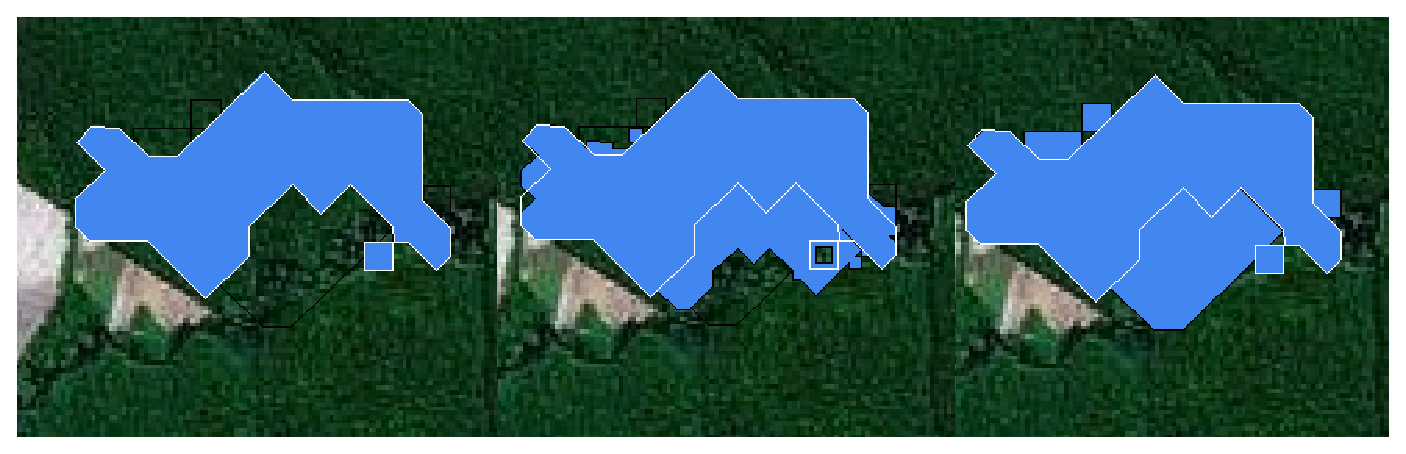
\includegraphics[width=0.9 \textwidth]{DeterUnit.eps}}
\subfigure{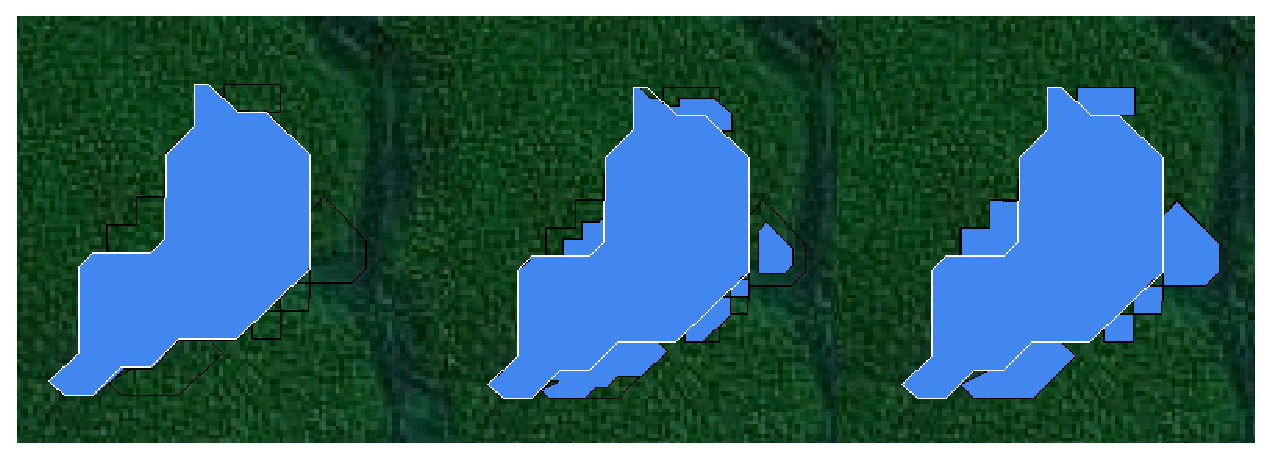
\includegraphics[width=0.9 \textwidth]{DeterUnit2.eps}}		\subfigure{\includegraphics[width=0.9 \textwidth]{DeterUnit3.eps}}		
	\caption[Region--Unit aus Deter--Daten]{Je drei Momentaufnahmen dreier Region--Units, die aus den Deter--Daten gewonnen wurden.\\\textit{\begin{tabular}{ll}
Quelle: &Luftbild, Google Maps;\\
&DETER-Daten dargestellt mit SECONDO
\end{tabular}}}
	\label{fig:RegionUnitDeter}
\end{figure}


%\section{Die Konstruktion der Moving-Regions}


\chapter[Ausblick ]{Ausblick} \label{Kapitel6}

\section*{Rückblick}

In der Einleitung, Kapitel~\vref{Kapitel1}, wurden zwei Beispiele für Moving--Regions gegeben und die Frage gestellt, ob es gelingen würde aus diesen Unwetter--Daten beziehungsweise den DETER--Daten kontinuierliche Bewegungen zu erzeugen. 

Zum ersten Beispiel kann nun gesagt werden, dass die Erzeugung prinzipiell gelingen würde (Falls das Beispiel nicht ein komplett fiktives wäre.). Jedoch würden bei Wetterdaten, die stark rotierende Daten sind die Probleme aus ~\vref{ProblemeRotation} zum Tragen kommen. In Abbildung~\vref{fig:Wetterdaten} wurde versucht, den Charakter von sich bewegenden Luftdruckgebieten zu treffen. Man kann gut sehen, dass die Interpolation zwar gelingt, das Ergebnis nach der Hälfte der Zeit aber viel zu groß ist und den beiden \textit{Faces} nicht stark ähnelt.

\begin{figure}
	\centering
	\includegraphics[scale=0.8]{Wetterdaten.eps}
	\caption[Bewegende Wetterdaten]{Fiktives Beispiel für bewegende Wetterdaten\\\textit{Quelle: Eigene Darstellung}}
	\label{fig:Wetterdaten}
\end{figure}
Beim zweiten Beispiel, den DETER--Daten, ist Überführung der Daten in eine kontinuierliche Form möglich, wie in Kapitel~\vref{Kapitel5} geschehen.


Auf dem Weg zur Lösung dieser Probleme wurden zwei verschiedene Applikationen erzeugt, das Java--Applet und die SECONDO--Algebra. 
Die Java-Applikation entstand nur aufgrund der Tatsache, dass es bereits eine solche Applikation gab, die von Erlend T\o{}ssebro entwickelt worden war. Diese Applikation wurde von dem Autor dieser Arbeit erweitert, so dass diese nun die Problemstellung der Arbeit löst. Obwohl diese Applikation nicht gefordert war, ist dieses Programm nicht überflüssig, es zeigt didaktisch gut aufbereitet wie das Matching passiert.

Die SECONDO--Algebra integriert die Möglichkeit zur Berechnung von kontinuierlichen Bewegungen in das SECONDO--System. Innerhalb dieses System ist es nun also möglich Regionen zu interpolieren. Aus technischen Gründen wurde dieser eine Operator als eigene Algebra implementiert, eine spätere Integration dieses Operators in die Moving--Region--Algebra ist aber möglich.




\section*{Probleme}
Sowohl bei der Bestimmung von Matchings mittels des Overlapping--Matches, als auch bei der Berechnung der entsprechenden Overlap--Bewertung, wird die Intersection--Funk"-tion der MakeOp-Klasse verwendet. Diese findet sich in der Plane--Sweep--Algebra. Leider führte die Verwendung dieser Funktion immer wieder zu Abstürzen, wie sie auch bei der Verwendung des \textit{union\_new} Operators derselben Algebra auftauchen. Deshalb wurde es leider nötig, auf diese Verfahren zu verzichten. Wenn die Probleme mit der externen Algebra behoben sind, kann man diese Verfahren einfach wieder reaktivieren, indem man in der Datei ,,RegionInterpolator.h'' die folgende Zeile wieder einkommentiert.
\begin{verbatim}
#define USE_OVERLAP
\end{verbatim}  

\section*{Erfahrungen}

In \vref{Zerlegung} wurde ein Algorithmus vorgestellt, der ein Polygon in konvexe Polygone zerlegen kann. Der Algorithmus wurde in der Hoffnung entwickelt, eine wesentlich weniger kleinteilige Zerlegung der Polygone zu erreichen, als das eine Triangulierung liefern würde. In der praktischen Erfahrung zeigt sich aber, dass die Zerteilung bei realen, komplizierten \textit{Faces} mit \textit{Holes} doch sehr kleinteilig wird. Abbildung~\vref{fig:ZerlegungFace2} zeigt ein solches Beispiel.

Die Verwendung dieses Algorithmus kann deshalb nicht uneingeschränkt empfohlen werden. Falls nicht klar ist, wie kompliziert die zu zerlegenden Polygone aufgebaut sind, so empfiehlt sich eher die Verwendung eines performanten Triangulierungs--Algorithmus. Ein solcher Algorithmus wird etwa unter \cite{Sei} vorgestellt.


\begin{figure}
	\centering
	\includegraphics[scale=0.9]{Convexer.svg.eps}
	\caption[Zerlegung eines Polygons, nur wenig besser als eine Triangulierung]{Ein Beispiel, in dem die Zerlegung eines Polygons Zerlegung liefert, die kaum besser als eine Triangulierung ist. Ein einziges Viereck ist das einzige vorkommende Polygon, das kein Dreieck ist.\\\textit{Quelle: Eigene Darstellung}}
	\label{fig:ZerlegungFace2}
\end{figure}

\section*{Raum für weitere Überlegungen}

Obwohl die implementierten Matchings bereits gute Ergebnisse liefern, kann man die entsprechende SECONDO--Algebra als Framework begreifen, um andere vielversprechende Matchings zu implementieren. Bei der Imlementierung der Algebra wie auch der Java--Applikation wurde auf eine guter Erweiterbarkeit geachtet, so dass eine Implementierung komplexerer Matching-Verfahren mit geringem Aufwand möglich ist. Es erscheint durchaus empfehlenswert, die eigenen Ideen zuerst in der Java--Applikation zu entwickeln, da diese viele Möglichkeiten des optischen Debuggen bietet. Im Anhang~\vref{eigeneMatch} wird beschrieben, wie man eigene Verfahren zum Matchen und Bewerten  implementieren, und wie man diese Verfahren in die Algebra einbauen kann.

Im Laufe der Arbeit wurden bereits einige Verfahren aufgezeigt, die eventuell gute Matches liefern können:
\begin{itemize}
\item Algorithmen zum Finden von pseudooptimalen Lösungen

In \vref{AARR} und \vref{AFRWW} wurden die Algorithmen aus den Veröffentlichungen \cite{AAR} und \cite{AFRW} vorgestellt. Diese Algorithmen könnten sehr gute Ergebnisse mit vertretbaren Aufwänden liefern. Da diese Paper aber eher aus dem Bereich der Mustererkennungen kommen, kümmern sich diese nur um 1:1 Matches.  Wie man mit diesen Algorithmen auf Vereinigungen und Zersplitterungen reagieren kann, muss noch überlegt werden.

\item Bewertung mittels $\min_{T\in\mathcal{T}}\delta(A,T(B))$

Das Verfahren, welches im letzten Abschnitt beschrieben wurde, liefert auch die Möglichkeit, gegebene 1:1 Matches zu bewerten. Eine diesbezügliche Implementierung wird voraussichtlich gute Ergebnisse bieten. 

\item statistisches Referenzpunktverfahren

In \vref{StatistikAlgo} wurde ein Verfahren aufgezeigt, das mittels statistischer Analyse aus einer Menge von Referenzpunkten zusammengehörige Cluster finden kann. Möglicherweise könnte dieses Verfahren gute Ergebnisse liefern, die Laufzeit wird aber nicht besonders gut sein.

\item Verfahren mit neuronalen Netzen oder mit Support--Vector--Maschinen

Unter \vref{neuroNetz} wurde auch ein Verfahren andiskutiert, das eine Gruppenbildung auf einer Menge von Referenzpunkten mittels neuronaler Netze oder Support--Vector--Maschinen durchführt. Weitere Überlegungen in dieser Richtung, zu Laufzeiten oder Qualitäten, wurden nicht angestellt. 
 
\item Maximize Overlap (set of cycles)

In \cite{TG} wird ein Matching--Verfahren entwickelt, das zwei Flächen matched, wenn Ihre Überlappung maximal ist. Dieses Verfahren ist unter Kapitel~\vref{MaxOver} näher beschrieben. Auch dieses Verfahren wurde nicht implementiert, könnte aber zu interessanten Ergebnissen führen.
\end{itemize}





\begin{appendix} \label{anhang}
\part*{Anhänge}
\mtcaddpart[Anh"ange]
\adjustptc[-2]
\parttoc

 
\chapter{Anleitung zur Benutzung des Java-Interpolators}\label{Handbuch}
\minitoc
\newpage
\section{Einleitung}
Im Rahmen meiner Diplomarbeit entstand, neben einer neuen Algebra f"ur SECONDO, auch eine Java-Anwendung, die die selbe Arbeitsweise wie die Algebra aufweist. Die Benutzung dieses Tools werde ich im Folgenden erl"autern.

Das Tool dient lediglich dem besseren Verst"andnis, wie die Algebra funktioniert. Ein Import oder Export mit SECONDO ist nicht m"oglich.
\section{Starten des Tools}
Das Tool ist in Java geschrieben, und wird als Jar-Datei verteilt. Um das Programm ausf"uhren zu k"onnen muss deshalb eine Java Laufzeitumgebung vorhanden sein. Ist dies der Fall, so l"asst sich das Programm mittels \begin{verbatim}
java -jar MCInterpolator.jar
\end{verbatim}  starten.

Es erscheint der Startbildschirm Abbildung \ref{fig:start}.

Dieser l"asst sich in vier Bereiche unterteilen:
\begin{itemize}
\item Eine Toolbar, die den Vrml-Export Button und den Zeit-Einsteller beinhaltet. 
\item Die Zeichen-Toolbar n"ahere Informationen zu dieser finden sich im Kapitel: ,,Zeichnen einer Region``
\item Der Zeichenbereich hier k"onnen Sie neue Regions zeichnen,und importierte Regions betrachten
\item Die Umschaltfl"achen, hier k"onne Sie zwischen den verschiedenen Werkzeugen wechseln. Nach dem Starten findet sich hier neben der Zeichenf"ache nur Konfigurationsschaltfl"ache, die im Kapitel: ,,Konfigurieren des Matchings`` n"aher beschrieben wird. Schlie"st man die Zeichnung von zwei Regions ab, so tauchen weitere Schaltfl"achen auf, die im Kapitel: ,,Die verschiedenen Ergebnisansichten`` erl"autert werden.
\end{itemize} 

\begin{figure}
   \centering
   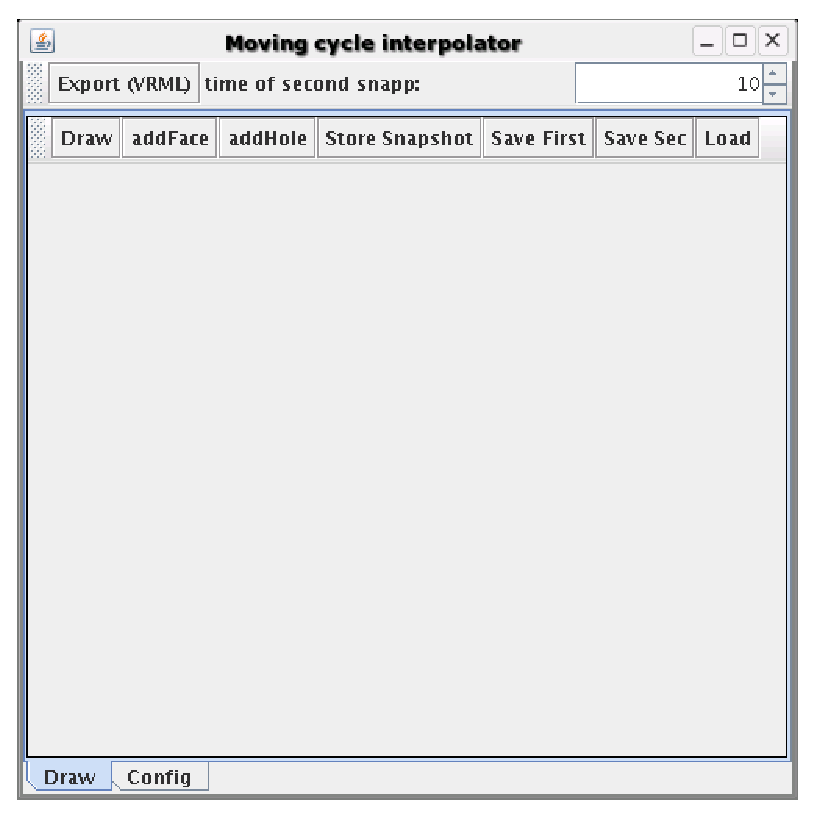
\includegraphics[scale=.8]{/home/java/Documents/Tex/Tex/start.eps}
   \caption{Der Startbildschirm}
   \label{fig:start}
\end{figure}

\section{Zeichnen einer Region}
\setcounter{section}{1}
Direkt nach dem Starten der Anwendung kann man anfangen, das erste Face zu zeichnen.  Das Zeichnen geht immer so vorsich, dass man die Punkte des Polygons nacheinander mit der Maus anklickt. Der neue Punkt, und die dazugeh"orige Linie werden direkt dargestellt. 

Das Polygon muss nicht geschlossen werden, aber bitte beachten Sie, dass alle Polygone einfache Polygone sein m"ussen. Eine entsprechende "Uberpr"ufung findet nicht statt.

Zum Zeichnen einer Region stehen folgende Werkzeuge bereit:
\begin{itemize}
\item Draw

Dieser Button l"oscht alle bereits eingegebenen Zeichnungen, und hinterl"asst ein leeres Zeichenblatt. Auch die eventuell bereits vorhandenen Schaltfl"achen f"ur die Ergebnissansichten werden ausgeblendet.
\item addHole

Hiermit kann man dem letzten Face ein Hole hinzuf"ugen. Holes unterscheiden sich von Faces darin, dass sie nicht blau sondern rot sind. Ein Hole muss komplett innerhalb seines Faces liegen, dies sicherzustellen ist die Aufgabe des Benutzers, eine "Uberpr"ufung findet nicht statt.
\item StoreSnapshot

Wollen Sie die Zeichnung einer Region beenden, so klicken Sie bitte auf diesen Button. Falls es der erste Schnappschuss ist, den Sie beenden, so f"arbt sich dieser blasser, und sie k"onnen den n"achsten zeichnen. Beenden Sie aber den Zweiten, so wird das passende Match berechnet, und in den zus"atzlichen Schaltfl"achen dargestellt, die Sie in ,,Die verschiedenen Ergebnisansichten`` finden.
\end{itemize} 
\section{Importieren- Exportieren}
Zum Importieren und Exportieren von Schnappsch"ussen, die Sie mit diesem Programm erzeugt haben stehen drei Schaltfl"achen zur Verf"ugung:

,,Save First``, ,,Save Sec`` und ,,Load``. Klicken Sie auf einen der beiden Save-Buttons, so "offnet sich ein Dateiauswahl-Dialog, in dem Sie einen Dateinamen f"ur die Schnappschuss-Datei angeben k"onnen.

Mit Hilfe des Load-Buttons k"onnen Sie dann diese SSchnappsch"usseeinzeln wieder laden. Falls Sie bereits zwei Schnappsch"usse in dem PProgrammhaben, so dr"ucken die bitte ,,Draw``, bevor Sie neue Dateien einlesen.
\section{Konfigurieren des Matchings}
Hinter der SSchaltfl"ache ,,Config`` verbirgt sich ein Dialogfenster (siehe Abbildung \ref{fig:Config}), in dem einige Einstellungen vorgenommen werden k"onnen:
\begin{itemize}
\item VRML Filename und VRML Application

Erl"auterungen zu diesen Feldern finden Sie in dem Unterkapitel: ,,Die verschiedenen Ergebnisansichten / Vrml-Export``
\item Auswahlfeld f"ur die Art des Matchings

Hier kann man ausw"ahlen, welches Matching man gerne ausf"uhren m"ochte. Die zur Zeit verf"ugbaren Matching-Methoden werden in der Arbeit ausf"uhrlich erl"autert.
\item Schieber f"ur die Parameter der Einzelmatches

Hier kann man einigen Einzel-Matches, zur Zeit dem OverlappingMatch und den Referenzpunktverfahren, einen Parameter "ubergeben. Bitte beachten Sie, dass dieser Parameter je nach der Art des Matches unterschiedliche Auswirkungen hat.
\item Schieber f"ur die Parameter des Optimalmatches

Das OtimalMatch setzt sich aus den EinzelMatches zusammen, indem es verschiedene Einzelmatches, mit verschiedenen Parametern, ausf"uhrt, und diese dann bewertet. In diese Bewertung flie"sen mehrere Kriterien gewichtet ein. Mit Hilfe dieser Schieber lassen sich die Gewichte der Einzel-Kriterien ver"andern.
\item Die Einzel-Bewertungen des Matches

In diesen Feldern finden Sie die Bewertungen des aktuellen Matches aufgeschl"usselt nach den einzelnen Kriterien.
\end{itemize} 
\begin{figure}
   \centering
   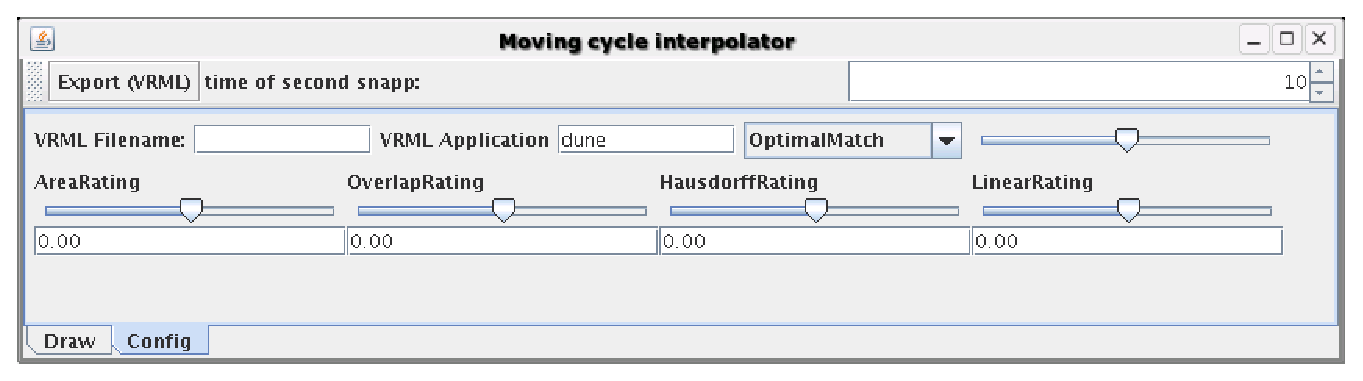
\includegraphics[scale=.65]{/home/java/Documents/Tex/Tex/Config.eps}
   \caption{Der Config-Dialog}
   \label{fig:Config}
\end{figure}
\section{Die verschiedenen Ergebnisansichten}
SoSobalder zweite ScSchnappschussbgeschlossen wird, erscheinen einige neue Schaltfl"achen, in denen Sie das Resultat des Matchings finden.

Bei den Erl"auterungen dieser Schaltfl"achen benutze ich die ScSchnappsch"ussesie in Abbildung \ref{fig:Splits} dadargestelltind.
\begin{figure}
   \centering
   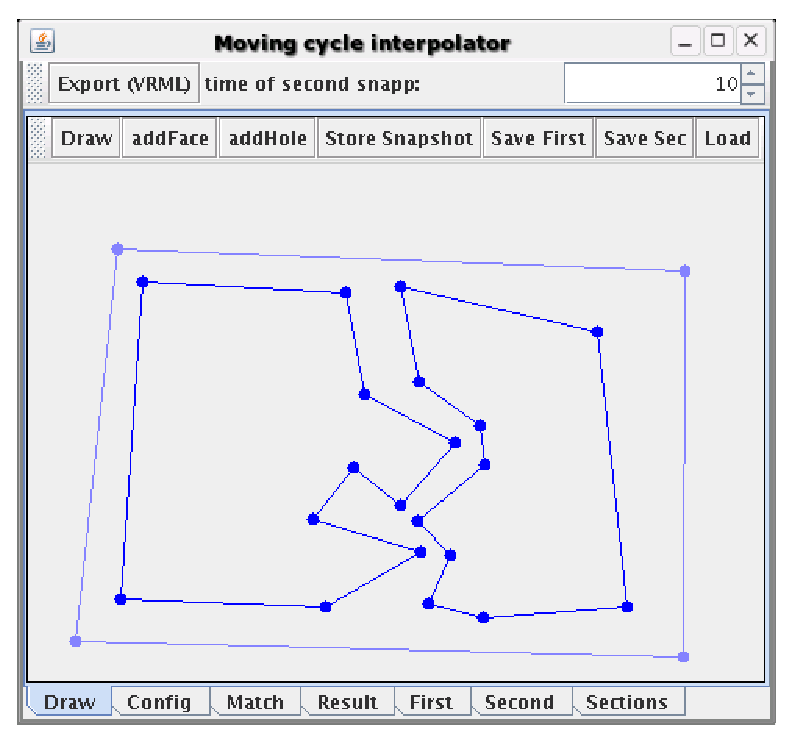
\includegraphics[scale=.8]{/home/java/Documents/Tex/Tex/Splits.eps}
   \caption{Das Beispiel}
   \label{fig:Splits}
\end{figure}
\subsection{Match}
In diesem Bildschirm (siehe Abbildung \ref{fig:Match}) finden Sie die beiden Schnappsch"usse in derselben Darstellung, wie in ,,First`` und ,,Second``. In dem entsprechenden Kapitel wird diese Darstellung n"aher erl"autert. 

W"ahlen Sie ein Element in einer der beiden Darstellungen aus, so wird das gematchte Element der anderen Darstellung selektiert. 

In der Rechten oberen Ecke des Fensters finden Sie den Namen des Matches, eine Erl"auterung zu diesem und die Bewertung in den Kategorien. Falls Sie ein OptimaMatch verwenden, so findet sich hier eine Liste mit allen Einzelmatches, die zu diesem ErErgebnisommen.
\begin{figure}
   \centering
   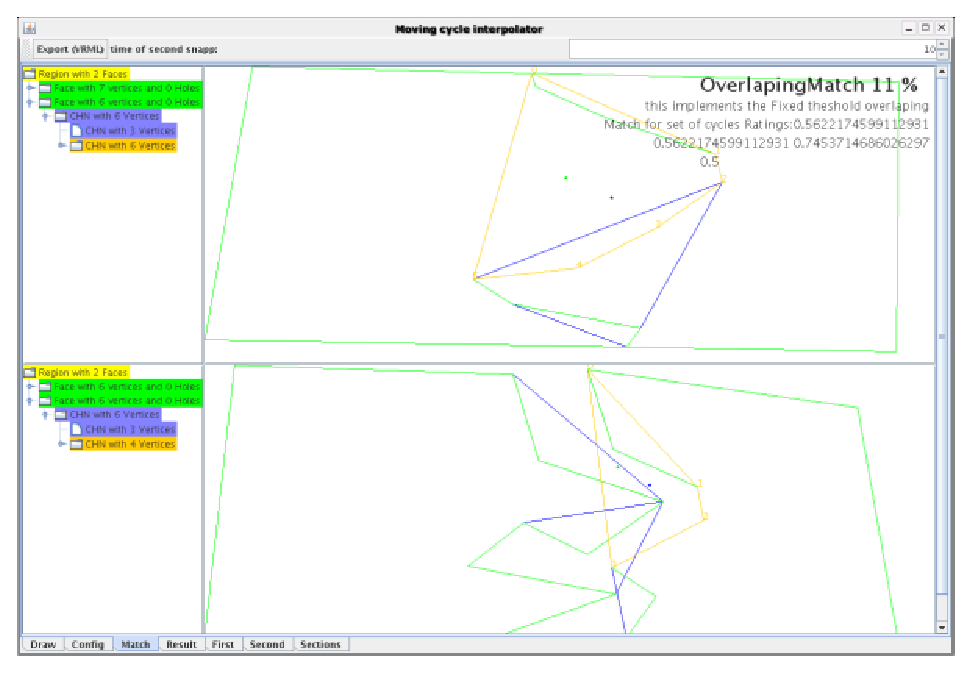
\includegraphics[scale=.8]{/home/java/Documents/Tex/Tex/Match.eps}
   \caption{Die Match-Darstellung}
   \label{fig:Match}
\end{figure}

\subsection{Result}
In diesem Bildschirm (siehe Abbildung \ref{fig:Result}) finden Sie eine isometrische Darstellung des Matches. Sie hier k"onnen Ihre bebeidenchnappsch"usse wiederfinden. Der Erste ist in blau gezeichnet, der Zweite in Rot. Die Linien, die die Beiden verbinden sind Grau. 

Mit Hilfe des Zeit-Einstellers in der obersten Toolbar k"onnen Sie den zweiten Schnappschusreiter nach hinten rechts verschieben, bzw. zur"uckholen. 

\begin{figure}
   \centering
   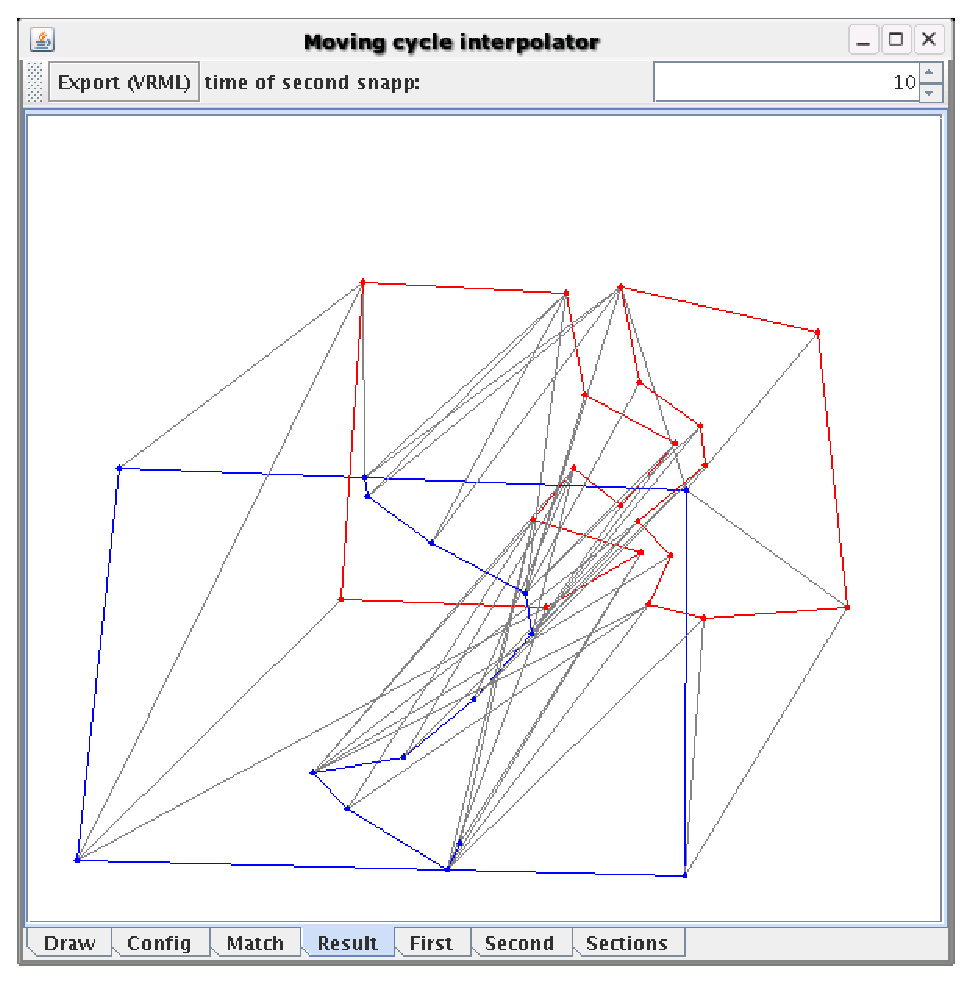
\includegraphics[scale=.6]{/home/java/Documents/Tex/Tex/Result.eps}
   \caption{Die Result-Darstellung}
   \label{fig:Result}
\end{figure}
\subsection{First und Second}
In dieser Ansicht (in Abbildung \ref{fig:Second} finden Sie ,,Second`` als Beispiel) finden Sie zwei Darstellungen des ConvexHullTrees eines Schnappschusses. Links finden Sie eine Baumansicht des ConvexHullTrees.

Diese Darstellung erm"oglicht es Ihnen, in dem Baum zu navigieren und Elemente zu selektieren. Mehrfachselektionen kann man vornehmen, indem man beim Klicken die Strg oder die UmUmschaltaste h"alt. Die einzelnen Elemente des Baumes sind farblich zu unterscheiden.

Die Farben bedeuten:
\begin{itemize}
\item Gelb Region
\item Gr"un Face
\item Blau ConvexHullTreeNode
\item Rot Hole
\item Orange Selektion
\end{itemize} 

Rechts finden Sie eine Darstellung des Baumes als Menge von Polygonen. Die Farbgebung entspricht der oben genannten, nur das die Region nicht extra dargestellt ist. Jedes Face ist durch das Polygon seines Cycles dargestellt, jedes Element eines ConvexHullTrees, einschlie"slich der Holes, ist durch seine konvexe H"ulle dargestellt. Selektiert man ein Element in der Baumansicht, so f"arbt sich dieses Orange, die Ecken der Konvexen H"ulle werden durchnummeriert und Schwerpunkt (blau) und Steiner-Punkt (gr"un) werden dargestellt.

\begin{figure}
   \centering
   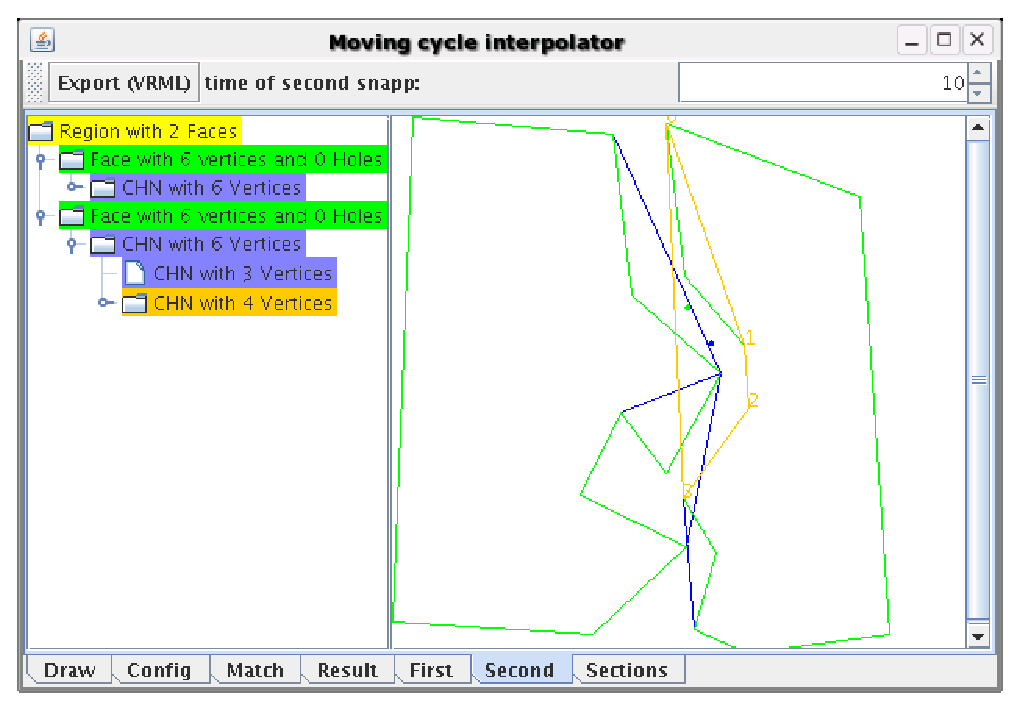
\includegraphics[scale=.8]{/home/java/Documents/Tex/Tex/Second.eps}
   \caption{Die ConvexHullTree-Darstellung des Zweiten Schnappschusses}
   \label{fig:Second}
\end{figure}
\subsection{Sections}
In dieser Darstellung (Abbildung \ref{fig:Sections}) finden Sie interpolierte Schnappsch"usse, die aus Ihrem Match erstellt wurden. In dem Feld mittig "uber der Darstellung k"onnen Sie w"ahlen, wieviele ScSchnappsch"usseie betrachten wollen. 

Diese tauchen dann in dem Zeichenbereich dieser Seite auf. Der Erste und der Letzte entsprechen dem ersten und dem zweiten Schnappschuss, den Sie eingegeben haben.
\begin{figure}
   \centering
   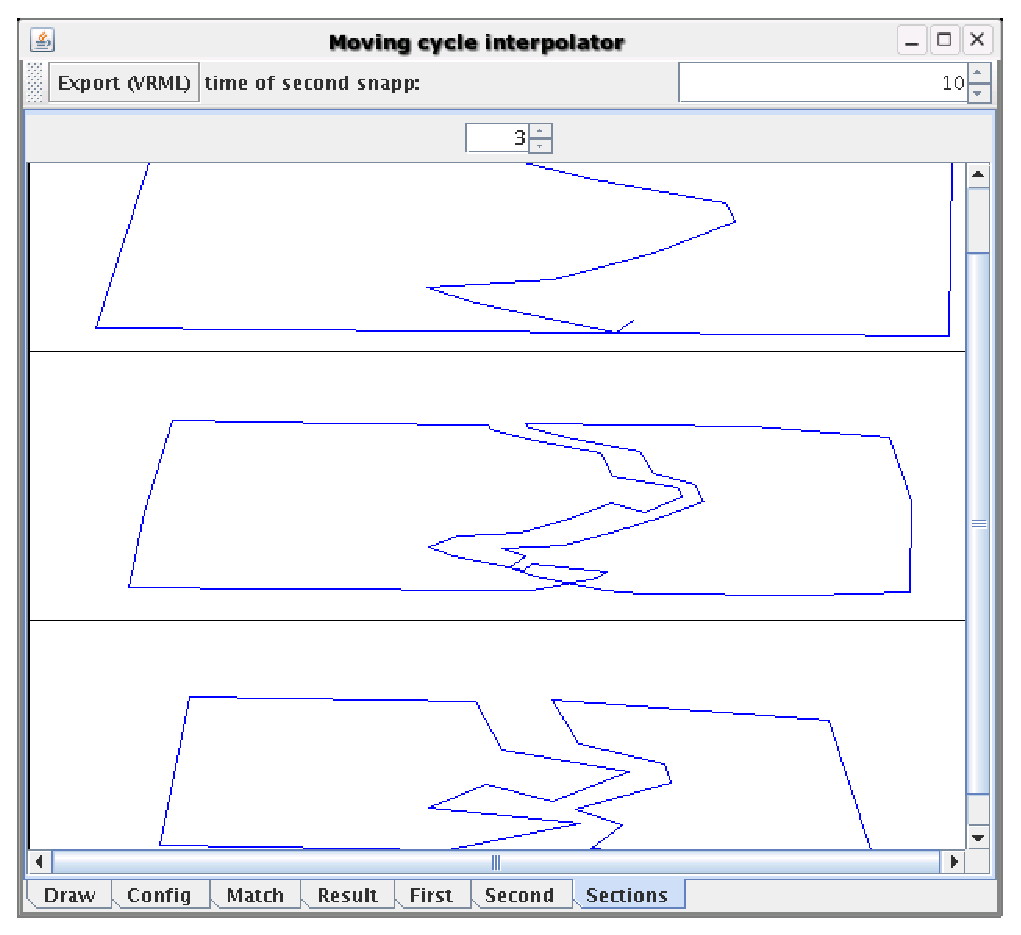
\includegraphics[scale=.8]{/home/java/Documents/Tex/Tex/Sections.eps}
   \caption{Drei Sections unseres Beispieles}
   \label{fig:Sections}
\end{figure}
\subsection{Vrml-Export}
Das Tool bietet die M"oglichkeit, ein Match in eine Vrml-Datei zu exportieren und so eine ansprechende 3D-Darstellung zu erhalten. Zu dem Vrml-Export geh"oren vier GUI-Elemente:
\begin{itemize}
\item VRML Filename im Config-Dialog

 In diesem Feld kann man den erw"unschten Dateinamen angeben, den die neue Vrml-Datei bekommen soll. Die Erweiterung .vrml wird automatisch ererg"anzt
\item VRML Application im Config-Dialog

Tr"agt man in diesem Feld einen Konsolenbefehl ein, mit dem man einen VRML-Viewer startet, so startet das Tool diesen Viewer direkt nach dem Export mit der neuen Datei.

\item Der ,,Zeit-Einsteller`` in der obersten Toolbar

Mit diesem Control k"onnen Sie die ,,H"ohe`` der 3D-Darstellung bestimmen. Kleine Werte f"uhren zu flachen Poyedern und Gro"se zu Hohen.
\item Der ,,Export (VRML)``-Button in der obersten Toolbar

Durch den Klick auf diesen Button wird der Export ausgel"ost. Die Vrml-Datei der gew"unschten H"ohe und mit dem gew"ahlten Namen wird erzeugt und direkt in dem Viewer Ihrer Wahl ge"offnet.
\begin{figure}
   \centering
   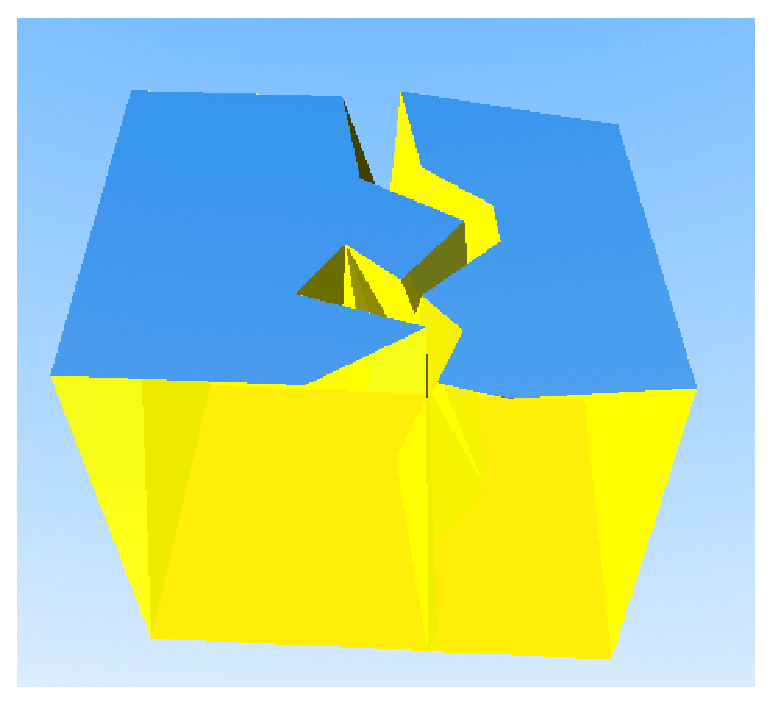
\includegraphics[scale=1]{/home/java/Documents/Tex/Tex/vrml.eps}
   \caption{Das Beispiel in einem Vrml-Viewer}
   \label{fig:vrml}
\end{figure}
\end{itemize}
  
 \chapter{Anleitung zur Implementierung eigener Matchings oder Ratings}\label{eigeneMatch}

\section{Die Implementierung eines Matches}

Ein eigenes Match muss von der abstrakten Klasse Match abgeleitet werden. Diese Klasse wird in \vref{MatchKlasse} näher beschrieben. Beim Erstellen des eigenen Matches müssen folgende Methoden implementiert werden:
\begin{itemize}
\item matchFaces
\item matchCHTNs
\item getBestMatch
\end{itemize}
Im Folgenden wird der Quellcode der Klasse \textit{CentroidMatch} betrachtet, um die Herangehensweise bei der Implementierung eigener Matches praktisch näher zu erläutern.

Zunächst wird der Konstruktor betrachtet:
\begin{lstlisting}[language=c++]
CentroidMatch :: CentroidMatch(RegionForInterpolation *source, RegionForInterpolation *target, double thresholdRel, bool useFinalize=true):
	Match(source, target, "CentroidMatch "+Utils :: toString( (int) (thresholdRel * 100)) + " %" , "this implements the position of centroids Match, known from the paper of Erlend Tossebro (5.2 1)")
{
    threshold = greatestDist * thresholdRel;                                
    addMatch(source, target);
    addMatch(target, source);
    matchFaces(source->getFaces(), target->getFaces());
    this->generateRatings();
    if(useFinalize)	    
    	finalize();
}
\end{lstlisting}
In dem Konstruktor wird zunächst der Superkonstruktor der Klasse Match aufgerufen. Dieser setzt \textit{source} und \textit{target}, benennt das neue Objekt und bereitet die Bewertung vor, indem der gemeinsame Durchmesser von \textit{source} und \textit{target} berechnet wird. Dann wird ein Match f"ur die Regionen \textit{source} und \textit{target} hinzugef"ugt und die Funktion \textit{matchFaces} mit allen Faces von source und target aufgerufen. Am Ende des Konstruktors muss die Funktion \textit{generateRatings()} aufgerufen werden. Diese berechnet die Bewertungen des Matches. Falls das Match nicht aus einem OptimalMatch aufgerufen wird, muss schlussendlich die Funktion \textit{finalize()} aufgerufen werden.

Die eben aufgerufene Funktion \textit{matchFaces()} kümmert sich darum, alle Matches von einzelnen Faces zueinander zu finden. Diese Funktion wird nun näher betrachtet. Auf die Betrachtung der Funktion \textit{matchCHTNs()} wird verzichtet, diese funktioniert analog.
\begin{lstlisting}[language=c++]
void CentroidMatch :: matchFaces(vector<Face*> *faces1, vector<Face*> *faces2)
{
	vector<Face*> unmatched;
	for(unsigned int i = 0; i < faces1->size(); i++)
	{
		for(unsigned int j = 0; j<faces2->size(); j++)
		{            
			double distance = getDistance(faces1->at(i)->getCycle(), faces2->at(j)->getCycle());
			if(distance < threshold)
			{
				addMatch(faces1->at(i), faces2->at(j));
				addMatch(faces2->at(j), faces1->at(i));
				addMatch(faces1->at(i)->getCycle(), faces2->at(j)->getCycle());
				addMatch(faces2->at(j)->getCycle(), faces1->at(i)->getCycle());
			}
		}
		unmatched.push_back(faces1->at(i));
	}
	for(unsigned int i = 0; i<faces2->size(); i++)
	{
		unmatched.push_back(faces2->at(i));
	}    
	while(!unmatched.empty())
	{
		Face *next = unmatched.back();
		unmatched.pop_back();
		vector<RegionTreeNode*> matches = getMatches(next);
		if(!matches.empty())
		{
			if(matches.size() > 1)
			{
				int dimMatch = 0;
				for(unsigned int i = 0; i < matches.size(); i++)
				{
					for(unsigned int j = 0; j<unmatched.size(); j++)
					{
						if(unmatched[j]->equals(matches[i]))
						{
							unmatched.erase(unmatched.begin() + j);
							break;
						}
					}                                       
					dimMatch += ( (Face*) matches[i])->getCycle()->getChildren()->size();
				}      
				matchCHTNs(next->getHolesAndConcavities(), getTargetChildren(next));	                
			}
			else
			{
				if(getMatches(matches[0]).size() > 1)
				{
					for(unsigned int i = 0; i < getMatches(matches[0]).size(); i++)
					{
						for(unsigned int j = 0; j < unmatched.size(); j++)
						{
							if(unmatched[j]->equals(getMatches(matches[0])[i]))
							{
								unmatched.erase(unmatched.begin() + j);
								break;
							}
						}                        
					}      
					matchCHTNs(( (Face*) matches[0])->getHolesAndConcavities(), getTargetChildren(matches[0]));
				}
				else
				{
					for(unsigned int j = 0; j<unmatched.size(); j++)
					{
						if(unmatched[j]->equals(matches[0]))
						{
							unmatched.erase(unmatched.begin() + j);
							break;
						}
					}   	
					matchCHTNs(next->getHolesAndConcavities(), getTargetChildren(next));                    
				}
			}
		}
	}
}
\end{lstlisting}


In den Zeilen~4~-~18 werden alle Kombinationen von Source- und Target-Faces durchgegangen. Falls ein Match gefunden wird, so werden die entsprechenden \textit{Faces} und die \textit{Cycles} der \textit{Faces} gematcht (in beiden Richtungen). In Zeile 17 werden außerdem alle Source-Faces dem Feld \textit{unnmatched} hinzugef"ugt.

In den Zeilen 19-22 ereilt dieses Schicksal auch alle Target-Faces, so dass in der Table jetzt alle \textit{Faces} der beteiligten \textit{Faces} zu finden sind.

Die Zeilen 19-78 werden solange durchlaufen bis \textit{unmatched} leer ist, also alle \textit{Faces} bearbeitet sind.

In den Zeilen 25-27 werden die Zuordungen vorgenommen:
\begin{itemize}
\item \textit{next} wird zum n"achsten, unbearbeiteten Face
\item \textit{next} wird aus \textit{unmatched} gel"oscht (\textit{next} wird ja gerade bearbeitet)
\item \textit{matches} werden die Targets von \textit{next}
\end{itemize} 

Falls \textit{matches} nicht \textit{null} ist, werden alle zu \textit{next} gematchten \textit{Faces} gesucht, aus \textit{unmatched} gel"oscht und es wird die Funktion \textit{matchCHTNs} mit den entsprechenden Kindelementen aufgerufen. Die mehrfache Verzweigung dieses Codeteiles resultiert daraus, dass \textit{next} auf mehreren Seiten eine 1:n Beziehung liegen k"onnte. 

Es muss noch die Methode \textit{getBestMatch()} in zwei Überladungen implementiert werden, so dass es eine solche Methode gibt, die mehrere \textit{Faces} als Eingabe bekommt und ein \textit{Face} zurückgibt und eine die dasselbe für \textit{ConvexHullTreeNodes} tut. Im Folgenden wird nur die Funktion für \textit{Faces} betrachtet, die andere funktioniert analog.
\begin{lstlisting}[language=c++]
Face *CentroidMatch :: getBestMatch(Face *source, vector<Face*> *targets)
{
	double best = numeric_limits<double> :: max();
	Face* bestMatch = NULL;    
	for(unsigned int i = 0; i < targets->size(); i++)
	{    	    	
		double dist = getDistance(source->getCycle(), targets->at(i)->getCycle());        
        	if(dist < best)
		{
            		bestMatch = targets->at(i);
            		best = dist;
		}
    	}    
    	return(bestMatch);
}
\end{lstlisting}
In dieser Funktion werden alle \textit{Faces} aus \textit{targets} mit dem \textit{source} verglichen. Dabei wird das \textit{Target}, dessen Schwerpunkt den geringsten Abstand zu dem Schwerpunkt von \textit{source} ermitttelt und zurückgegeben.

\section{Die Integration eigener Matches in das Optimal Match}

Hat man ein eigenes Match implementiert, so muss man dieses auch in das \textit{OptimalMatch} eingehen lassen, da die SECONDO--Algebra nur dieses Match ausführt. Das \textit{OptimalMatch} beinhaltet im Wesentlichen nur den Konstruktor:
\begin{lstlisting}[language=c++]
OptimalMatch::OptimalMatch(RegionForInterpolation *source, RegionForInterpolation *target,vector<double> weights):
Match(source->clone(),target->clone(),"","")
{	        
	double AreaWeight = weights[0];
	double OverlapWeight = weights[0];
	double HausdorffWeight = weights[0];
	double LinearWeight = weights[0];
	Match *best;
	vector<Match*> candidates;
	candidates.push_back(new OverlapingMatch(source->clone(),target->clone(),0.3,false));
	candidates.push_back(new SteinerPointMatch(source->clone(),target->clone(),0.3,false));
	candidates.push_back(new CentroidMatch(source->clone(),target->clone(),0.3,false));
	best=candidates[0];
	for(unsigned int i=1;i<candidates.size();i++)
	{
		if(candidates[i]->getRating(AreaWeight,OverlapWeight,HausdorffWeight,LinearWeight)==best->getRating(AreaWeight,OverlapWeight,HausdorffWeight,LinearWeight))
		{            	
			best->addName(candidates[i]->getName());
		}
		if(candidates[i]->getRating(AreaWeight,OverlapWeight,HausdorffWeight,LinearWeight)>best->getRating(AreaWeight,OverlapWeight,HausdorffWeight,LinearWeight))
best=candidates[i];
	}
	best->finalize();
	this->name=best->getName();
	this->source=best->getSource();
	this->target=best->getTarget();
	this->description=best->getDescription();
	this->Arearating=best->getAreaRating();
	this->Hausdorffrating=best->getHausdorffRating();
	this->linearRating=best->getLinarRating();
	this->Ovelaprating=best->getOverlapRating();
	this->maps=best->getMaps();
}		
\end{lstlisting}
Zu Anfang des Konstruktors wird ein Feld angelegt, in dem alle Kantdaten für ein gutes \textit{Match} stehen. Neue \textit{Matches} müssen hier eingetragen werden. Dieses Feld wird dann nach dem am bestem bewerteten \textit{Match} durchsucht. Dieses \textit{Match} wird finalisiert und seine Attribute in das \textit{OptimalMatch} kopiert.

\section{Die Implementierung eigener Ratings}

Die Ratings dienen dazu, aus den verschiedenen Kanidaten für eine OptimalMatch den Besten herauszufinden. Implementiert man ein neues Rating, so kann man passendere Matches finden. 

In der Datei ,,Match.h'' finden sich die Attribute:
\begin{lstlisting}[language=c++]
protected:
	double Hausdorffrating;
	double Ovelaprating;
	double Arearating;
	double linearRating;
 \end{lstlisting}
Um ein eigenes Rating zu implementieren, muss man die Liste von Attributen erweitern. Zu den eigenen  Attributen muss man dann die Methode anlegen, die diese auslesen wie etwa:
\begin{lstlisting}[language=c++]
double Match :: getAreaRating()
{
    return(Arearating);
}
\end{lstlisting}

In der Datei ,,Match.cpp'' findet sich die Methode \textit{getRating}, die die gewichtete Summe aller Ratings zurückliefert. Auch diese Methode muss um das neue Rating erweitert werden.

In den Zeilen 4~--~7, des Konstruktors des OptimalMatches,  werden die einzelnen Gewichte aus dem übergebenen Feld gelesen, in  der Zeile~16 wird die gewichtete Summe gebildet und  in  28~--~31 werden die Ratings des besten Kanidaten in das OptimalMatch kopiert. Auch  diese Stellen müssen um das eigene Rating erweitert werden.

In der Datei ,,RegionInterpolator.cpp'' befindet sich die Präprozessoranweisung, die die Anzahl der zu übergebenden Gewichte angibt.
\begin{lstlisting}[language=c++]
#define COUNTWEIGHT 4
[...]
static int interpolateValueMap_1(Word* args,
                        Word& result,
                        int message,
                        Word& local,
                        Supplier s) 
{                         
    result = qp->ResultStorage(s);
    Region* reg1 = (Region*) args[0].addr;
    Region* reg2 = (Region*) args[1].addr;
    Periods *range = ((Periods*)args[2].addr);
    const Interval<Instant> *inter;    
    range->Get( 0, inter );
    assert(inter->IsValid());
    RegionForInterpolation *reginter1=new RegionForInterpolation(reg1);
    RegionForInterpolation *reginter2=new RegionForInterpolation(reg2);
    vector<double> weigths = vector<double>(COUNTWEIGHT);
    weigths[0] = 0.7; 				// AreaWeight
    weigths[1] = 0.7;				// OverlapWeight
    weigths[2] = 0.5;				// HausdorffWeight
    weigths[3] = 1.0;				// LinearWeight
    Match *sm=new OptimalMatch(reginter1,reginter2,weigths);
    mLineRep *lines=new mLineRep(sm);    
    URegion *res= new URegion(lines->getTriangles(),*inter);
    result.addr=res->Clone();       
    return 0;
}
\end{lstlisting}
In der Value--Mapping--Funkion, die den Aufruf ohne übergebene Gewichte abwickelt, werden die Gewichte auf Standard--Werte gesetzt. (Zeilen~19~--~22) Auch diese Stelle muss angepasst werden, genauso wie die Spezifikation des Operators. 

Um die bislang enthaltenen Ratings zu berechnen, wird die Methode \textit{generateRatings()} benutzt. Dieser wird nun näher beschrieben, da dies auch bei der Implementierung neuer Ratings helfen kann.
\begin{lstlisting}[language=c++]
void Match :: generateRatings()
{
	Hausdorffrating = 0.0;
	Ovelaprating = 0.0;
	Arearating = 0.0;
	linearRating = 0;
	NrOfRatings = 0;
	for(int i = 0; i < source->getNrOfFaces(); i++)
	{    		
		vector<RegionTreeNode*> tmp = getMatches(source->getFace(i));
		if(tmp.size() == 0)
		{        
			Hausdorffrating += Utils::getDiameter(Utils :: convertCHLine2LineWA(source->getFace(i)->getCycle()->getLines()));
			Ovelaprating += 0.0;
			Arearating += 0.0;
			linearRating += 0.5;
			NrOfRatings++;
		}
		else
		{                        
			rateFace(source->getFace(i), tmp);            
		}         
	}
	[...]
	Arearating = Arearating / NrOfRatings;
	Ovelaprating = Ovelaprating / NrOfRatings;
	Hausdorffrating = 1 - Hausdorffrating / NrOfRatings / greatestDist;
	linearRating = linearRating / NrOfRatings;            
}	
\end{lstlisting}
Nachdem die verscheidenen Variablen initialisiert wurden, Zeile 3~--~ 7, werden alle \textit{Faces} der Source--Region durchlaufen. Wird ein betrachtetes \textit{Face} gegen $null$ gematcht, so werden die Variablen auf den entsprechenden Wert gesetzt. Ansonsten wird die Funktion \textit{rateFace()} aufgerufen, in der die weitere Berechnung für einzelne \textit{Faces} stattfindet. 

In Zeile 24 passiert dasselbe für die Target--Region (hier nicht dargestellt). Zuletzt werden die einzelnen Ratings endgültig berechnet. Meist geschieht das, indem die Summe der Einzelratings duch deren Anzahl dividiert wird. 

In den Methoden \textit{rateFace()} und \textit{rateCHTN()} werden die Einzelratings berechnet. Die Berechnung passiert analog zu der Berechnung in \textit{generateRatings()}.


 \chapter{Klassendiagramm}
 \begin{landscape}
 
 \begin{figure}	
	\includegraphics{Klassen.1}
	\caption{Klassendiagramm mit allen Klassen}
	\label{fig:UML_Klassendiagramm}
\end{figure}

\end{landscape}
 \begin{figure}	
	\includegraphics{Klassen.6}
	\caption{Die Klasse LineWA}
	\label{fig:UML_LineWA}
\end{figure}

 \begin{figure}	
	\includegraphics{Klassen.7}
	\caption{Die Klasse CHLine}
	\label{fig:UML_CHLine}
\end{figure}

 \begin{figure}	
	\includegraphics{Klassen.8}
	\caption{Die Klasse LineDist}
	\label{fig:UML_LineDist}
\end{figure}

 \begin{figure}	
	\includegraphics{Klassen.13}
	\caption{Die Klasse PointWNL}
	\label{fig:UML_PWNL}
\end{figure}

 \begin{figure}	
	\includegraphics{Klassen.2}
	\caption{Die Klasse ConvexHullTreeNode}
	\label{fig:UML_CHTN}
\end{figure}


 \begin{figure}	
	\includegraphics{Klassen.4}
	\caption{Die Klasse Face}
	\label{fig:UML_Face}
\end{figure}

 \begin{figure}	
	\includegraphics{Klassen.5}
	\caption{Die Klasse Region}
	\label{fig:UML_Region}
\end{figure}

 \begin{figure}	
	\includegraphics{Klassen.3}
	\caption{Die Klasse RegionTreeNode}
	\label{fig:UML_RTN}
\end{figure}

\begin{figure}	
	\includegraphics{Klassen.9}
	\caption{Die statische Hilfs-Klasse Utils}
	\label{fig:UML_Utils}
\end{figure}

\begin{figure}	
	\includegraphics{Klassen.10}
	\caption{Die Klasse SingleMatch}
	\label{fig:UML_SingleMatch}
\end{figure}

\begin{figure}	
	\includegraphics{Klassen.11}
	\caption{Die Klasse Match}
	\label{fig:UML_Match}
\end{figure}

\begin{figure}	
	\includegraphics{Klassen.12}
	\caption{Die Klasse CentroidMatch}
	\label{fig:UML_CMatch}
\end{figure}


\begin{figure}	
	\includegraphics{Klassen.14}
	\caption{Die Klasse SteinerPointMatch}
	\label{fig:UML_SMatch}
\end{figure}

\begin{figure}	
	\includegraphics{Klassen.15}
	\caption{Die Klasse OverlapingMatch}
	\label{fig:UML_OMMatch}
\end{figure}

\begin{figure}	
	\includegraphics{Klassen.17}
	\caption{Die Klasse OptimalMatch}
	\label{fig:UML_OptimalMatch}
\end{figure}


\begin{figure}	
	\includegraphics{Klassen.16}
	\caption{Die Klasse mLineRep}
	\label{fig:UML_mLineRep}
\end{figure}



 
\chapter{Quelltexte}
\minitoc
\newpage
\begin{landscape}
\section{ConvexHullTreeNode}
\begin{tiny}
\lstinputlisting[multicols=2,numbers=none]{ConvexHullTreeNode.java}
\end{tiny}
\end{landscape} 
  
 \printindex
 \addcontentsline{toc}{chapter}{E $\:$ Stichwortverzeichnis}
 \setcounter{chapter}{5}
\bibliography{literatur}

\bibliographystyle{geralpha}
\listoffigures
\include{Erklaerung}
 \end{appendix}


\end{document}